%------------------------------------------------Main.tex % the one that you should compile ;)

\documentclass[a4paper,12pt,oneside]{report}

%------------------------------------------------packages
\usepackage{array,multirow,makecell}
\usepackage{setspace}
\usepackage{bibtopic}
\usepackage{ulem}
\usepackage[utf8x]{inputenc}
\usepackage[T1]{fontenc}
\usepackage{graphicx}
\usepackage{listings}
\usepackage{titling}
\usepackage{url}
\usepackage{titlesec}
\usepackage{marvosym}
\usepackage{tabularx}
\usepackage[top=3cm,bottom=3cm,left=2cm,right=2cm]{geometry}
\usepackage{fancyhdr}
\usepackage{enumitem}
\usepackage{amsfonts}
\usepackage{soul}
\usepackage[square, numbers, comma, sort&compress]{natbib}
\usepackage{xcolor}
\pagestyle{fancy}
\renewcommand{\headrulewidth}{3pt}
\newcommand{\horrule}[1]{\rule{\linewidth}{#1}} % Horizontal rule
\usepackage{pifont} %----for customized item label
\setlength{\headheight}{15pt} 
\usepackage{version}  %----to use \begin{comment}
\setlength{\parskip}{0.7em}   %--espace entre paragraphes
\usepackage{lettrine} %----first big letter 
\usepackage[french,english]{babel}
\usepackage{verbatim}
%---------------------------------------------------more packages
\usepackage{ulem}
\newcommand{\HRule}{\textcolor{lightgray}{\rule{15.5 cm}{0.12 cm}}}
\newcommand{\Hrule}{\textcolor{lightgray}{\rule{13.5 cm}{0.15 cm}}}


\fancyhead[L]{}
%-------------------- interligne
\renewcommand{\baselinestretch}{1.3}


\usepackage[section]{placeins}

%------------------------------format du titre de section
\titleformat{\section}[block]
  {\huge\bfseries}
  {\color{gray} \thesection
   \hspace{10pt}\vline}
  {10pt}
  {}


\newcommand{\customizeNumber}{%
  \fontsize{40}{40}\usefont{U}{eur}{b}{n}}

\newcommand{\chapterNumberr}{%
  \fontsize{12}{12}\usefont{U}{b}{n}}



%---------------------------------------------Here We Go !
\begin{document}


%---------------------------------------------Front Page
%input{start/front.tex}
%----------------------------------------------Abstract, Signatures, Acknowledgement

%---------------------------------------environment abstract
\newenvironment*{resume}{%
\renewcommand*{\abstractname}{\begin{center}\Huge \textbf{Abstract}\end{center}}
\begin{abstract}
{\end{abstract}}

%---------------------------------------environment signatures
\newenvironment*{Signatures}{%
\renewcommand*{\abstractname}{\Huge \textbf{Signature}}
\begin{abstract}
}{\end{abstract}}

%---------------------------------------environment acknowledgment
\newenvironment*{acknowledgement}{%
\renewcommand*{\abstractname}{\begin{flushleft}\Huge \textbf{Acknowledgement}\end{flushleft}}
\begin{abstract}
}{\end{abstract}}



%=================================================================================
%---------------------------------------------Abstract
\begin{resume}
\bigskip

\lettrine[lines=2]{T}his report covers the design and the development of a web component included in a automated fleet dispatching solution.

This component enables the back end user, which is the SaaS Office, to view and control drivers in real time. Moreover, it allows him to inspect and study the rides booked by the SaaS company's users.

This project is achieved as second year's design and development project at the National School of Computer Science.

Keywords: Javascript, Google Maps Api, AngularJS, UI, Bootstrap, ui-grid, ng-map...

\end{resume}
%-------------------------------------------Signature
\begin{center} 
\begin{Signatures}

%\includegraphics[height=3 in]{images/acknowledgment_Grati.png}
%\includegraphics[height=3 in]{images/acknowledgment_Faten.jpg}
\end{Signatures}
\end{center}
%----------------------------------------- Acknowledgement
\begin{acknowledgement}


{

\bigskip
\lettrine[lines=2]{I}n conducting this report, we have received meaningful assistance from many quarters which we
like to put on record here with deep gratitude and great pleasure.


First and foremost, we express our sincere gratitude to our supervisor,  Mohamed Ali Charmi, who extended his complete support and helped to make us deliver our best, as well as our co-workers for their guidance and valuable pieces of advice during different phases of the elaboration of the project.
Simply put, we could not have done this work without the amount of help and trust we received from them. We appreciate their patience in checking and reviewing our work.
\bigskip

We would also like to thank all of our teachers at the National School of Computer Science for their continuous help and treasurable training during our study years.

Finally, special thanks to the jury members who honored us by examining and evaluating this modest contribution.}
\end{acknowledgement}


\pagenumbering{roman}
%------------------------------------------ Contents


{
\setcounter{secnumdepth}{3}
\setcounter{tocdepth}{4}
\renewcommand{\contentsname}{Contents} % Dans le corps du document,avant la commande \tableofcontents.
\tableofcontents}


%--------------------figures
{\listoffigures}


%---------------------tables--------minimum=4
{\listoftables } 



%-------------------- Acronyms
\chapter*{Glossary of Acronyms}
\addcontentsline{toc}{chapter}{Glossary of Acronyms} % to add it to the tables of contents


~~~~~\textbf{SaaS : } Software as a Service

\textbf{API : } Application programming interface, a particular set of rules (’code’) and specifications that software programs can follow to communicate with each other.

\textbf{VTC : } 'Véhicule de Tourisme avec Chauffeur' : Tourist Vehicle with Driver

\textbf{SPA : } Single Page Application

\textbf{JSON : }JavaScript Object Notation

\textbf{HTML : } HyperText Markup Language is the main markup language for displaying web pages and other information that can be displayed in a web browser.

\textbf{CSS : }Cascading Style Sheets is a style sheet language used to describe the presentation semantics (the look and formatting) of a document written in a markup language

\textbf{JS : } JavaScript is a dynamic prototype-based scripting language , used in the form of client-side in order to give enhanced user interfaces and dynamic websites.

\textbf{MVC : } Model-View-Controller is a design pattern for successfully and efficiently relating the user interface to underlying data models. 

\textbf{DOM : } Document Object Model is a cross-platform convention for creating a fully dynamic HTML.

\textbf{UI : } User Interface



\pagenumbering{arabic}


%------------------------------------------ General Introduction
\chapter*{General Introduction}
\addcontentsline{toc}{chapter}{General Introduction} % to add the intro to the tables of contents



\lettrine[lines=2]{I}n the era of constant evolution, new technologies are being released every day in order to satisfy human being's need for fast and efficient services.

% general needs of security 
%---------The frantic pace at which websites and mobile applications deliver utilities nowadays furthers users' expectations and makes their lives easier.  Nevertheless, it affects users' patience and allows them to become particularly choosy and critical. To the extend of, in several cases, users seeking for reliable services, prefer instant and rapid paid services over slow free ones.
In today's competitive market, responsiveness to customer or supplier demand is often a decisive factor in the success of an organization. The network is considered one of the most critical resources in an organization, both in the private and public sectors.

Connecting your network to the Internet provides access to an enormous amount of information and allows you to share information on an incredible scale. However, the communal nature of the Internet, which creates so many benefits, also offers malicious users easy access to numerous targets. The Internet is only as secure as the networks it connects, so we all have a responsibility to ensure the safety of our networks.

%Especially in daily activities, citizens can not afford to invest a lot of time into transport. Businessmen, daily workers and even tourists have a busy schedule and follow a strict plan. A lot of people arrange a detailed proposal on how to spend the day as they must respect that scheme.   
%---------------------------------
In this context, an automated network security monitoring solution fits as the best option for an organization. The aim of this project is to enable security analysts to monitor network availability, integrity and confidentiality. Detect malicious activity even before it happens.

Our work is presented throughout this report accordingly to the following plan. In the first chapter, we describe the general frame of the project by introducing the host company, going through its main highlights, then presenting the project overview. Throughout the second chapter, we shed the light on some of the most important keywords of our work and provide a brief literature review. Then we study the existing solution, evaluate its efficiency and present our solution. In the third chapter, we make a list of the functional and the non-functional requirements related to our application. In addition, we present several use case diagrams to clarify the features of our solution. In the fourth chapter, we describe the application's architecture and its design. In the fifth chapter, we detail the description of the different technologies used to build the project and present the main interfaces using screen-shots.

Finally, we conclude our work by giving future prospects and potentials upgrades for our application.
\thispagestyle{empty}


%------------------------------------------chapter1 General Context

\chapter{General Context}
\renewcommand{\chaptername}{Chapter}
This chapter introduces the general context of the conducted work. 
We start by presenting the hosting company, describing its line of work and enumerating its clients. Afterwards, we proceed by relating the goal of our project as well as the expected results.

\section {Presentation of the hosting company}

Through this section, we present the hosting company and enlist the different phases of its evolution.

\subsection{ATHENA Experts}

%We define different terms and clarify various concepts about the company. As a matter of fact, WebForge delivers SaaS product in association with Classnco. The product is called YusoFleet, and each client uses this solution according to his preferences.  
ATHENA is a service company specialized in Information Security and governance. Since 2007, ATHENA is supporting its clients in technical, operational and organizational aspects related to its specialization areas. Operating internationally, ATHENA already has 4 branches in :
\begin{itemize}
\item Paris (France)
\item Bucharest (Romania)
\item Tunis (Tunisia)
\item Kinshasa (Democratic Republic of Congo)
\end{itemize}
Driven by a growing development, ATHENA intends to strengthen its international presence in order to be closer to its clients.
%\begin{itemize}[label=\ding{217}]\item \textbf{WebForge Technologies SARL}Webforge Technologies SARL is a Tunisian startup that develops innovative solutions for urban transport. It is in fact a subsidiary company of Classnco.


%\item\textbf{Classnco}Launched in 2012, the Parisian start-up Class \& Co is developing its first stream optimization software for the transport of persons. The company designs, develops and markets software for a SAAS existing transport stakeholders on demand.It provides them with technology solutions that automate and optimize certain key business processes including booking, dynamic management of drivers schedules and other operations (reporting shopping, billing, ...).

%\item 
%\textbf{YusoFleet}

%YusoFleet is the first digital solution to facilitate the activity of radio taxis, ambulance and VTC. The main idea is to offer a unique and simple tool for scanning reservation management, as well as exchanges with customers and drivers.

%Two years after its founding, they connect today approximately 5,000 vehicles and performed almost 500,000 automatic dispatchs successfully. They equip fleets of 3 vehicles to 1000 and, for example, this software is used by leading motorcycle taxi in Paris. \cite{linkedin}



%\end{itemize}


\subsection{Provided services }

\subsubsection{PCI DSS}
ATHENA supports its clients with PCI DSS (Payment Card Industry Data Security Standard) approach and offers the following services :
\begin{itemize}
\item PCI DSS training. 
\item Supports in the scoping study and defining the scope of your PCI DSS certification project.
\item Supports in PCI DSS compliance and mainting of the certification
\item Recurrent Audits of your PCI DSS scope.
\item Mock Audit to prepare for PCI DSS certification.
\end{itemize}
\subsubsection{Audit}
ATHENA offers a comprehensive set of IT security audits, including :
\begin{itemize}
\item Infrastructure Penetration Testing.
\item Wireless Penetration Testing.
\item Application Penetration Testing.
\item Social Engineering Penetration Testing.
\item Source code security audit.
\item Technical Audit.
\item Configuration Audit.
\item Compliance Audit.
\item Recrrent Audit.
\end{itemize}
\subsubsection{Consulting}

ATHENA leverages an extensive knowledge of the IT security field to offer the following consulting services :
\begin{itemize}
\item Risk Analysis.
\item Development/review of security policies.
\item Secure architecture design.
\item Technical and technological study and advise.
\item Information Security Management System (ISMS) implementation assistance.
\item Chief Information Security Officer (CISO) assistance/coaching.
\item Project management assistance.
\end{itemize}
\subsubsection{Deployment}
Through the following services, ATHENA assists its clients in setting up and developing a secure and efficient information system that meets the ever-growing requirements of the final users while respecting compliance obligations :
\begin{itemize}
\item Design of secure solutions.
\item Deployment of secure solutions.
\item Testing of information system proper operations.
\item Technical trainings and skills transfer.
\end{itemize}
Key Solutions deployed by ATHENA :
\begin{itemize}
    \item SIEM (Security information and event management).
    \item DLP (Data Loss Prevention).
    \item Data Encryption and Digital Signature.
    \item VMS (Vulnerability Management System).
    \item Endpoint Detection and Response.
    \item Next Generation Firewalls.
    \item Digital forensics.
    \item SOC (Security Operations Center).
\end{itemize}
\begin{figure}[!htpb]
\begin{center}

\includegraphics{images/ATHENAdeployment.png}
\caption{ATHENA's deployed solutions}
\label{schema}
\end{center}
\end{figure} 
\subsubsection{Digital Forensics}
ATHENA's digital forensics team addresses potential security incidents as well as malicious cyber-attacks via the following services :
\begin{itemize}
    \item Trackback of the cyber-attack or the security incident.
    \item Collection and preservation of relevant evidence.
    \item Intruders identification.
    \item Assessment of the damage's extent.
    \item Protection against attack renewal.
\end{itemize}
\begin{figure}[!htpb]
\begin{center}

\includegraphics{images/ATHENAdigitalf.png}
\caption{Encase's Logo}
\label{schema}
\end{center}
\end{figure} 
\subsubsection{Managed Services}
Thanks to ATHENA's Security Operation Center (SOC), ATHENA remotely provides its clients with the following services:
\begin{itemize}
    \item Real time monitoring of services and equipment.
    \item Logs collection and correlation.
    \item Real time security events management.
    \item Hotline and incident management.
    \item Performances monitoring.
    \item Administration and exploitation of services and equipment.
    \item Vulnerability management.
    \item Compliance tests.
    \item Data Leak Prevention.
\end{itemize}
\subsubsection{Business Continuity / Disaster Recovery Plan}
In order to ensure the continuity / quick and efficient recovery of its clients business in case of a disaster, ATHENA offers the following services :
\begin{itemize}
    \item Development of Business Continuity Plan (BCP) and/or Disaster Recovery Plan (DRP).
    \item Implementation of the BCP and/or DRP.
    \item Evaluation of the BCP and/or DRP efficiency and adequacy with the context of the client and the enforced regulations.
    \item Optimization of the "Efficiency / Cost" rate of the BCP and DRP.
    \item Disaster simlation.
\begin{figure}[!htpb]
\begin{center}
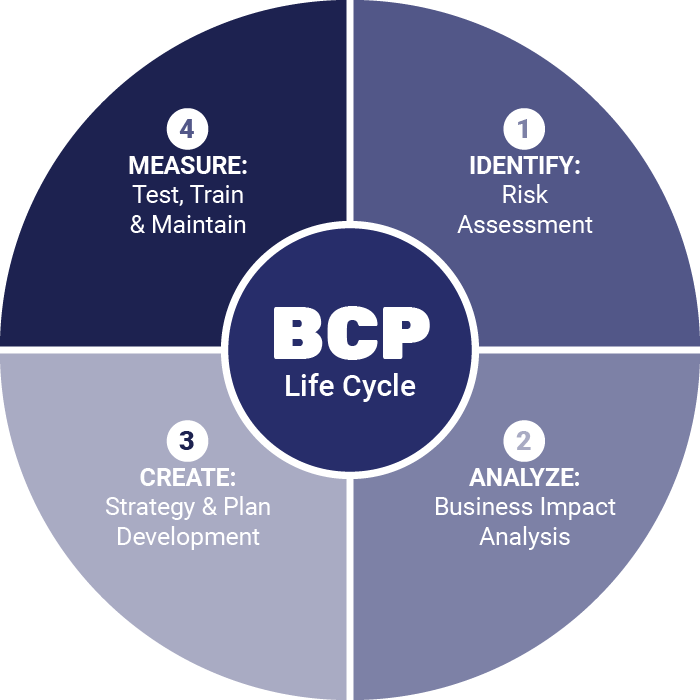
\includegraphics[ height=1.9 in]{images/ATHENABCP.png}
\caption{Business Continuity Plan}
\label{schema}
\end{center}
\end{figure} 
\end{itemize}

\subsubsection{Training and Awareness}
ATHENA offers a comprehensive range of training that cover various aspects of information security. These training courses are specifically adapted to the context, the business needs as well as the constraints of the client.
ATHENA's training covers four main areas :
\begin{figure}[!htpb]
\begin{center}

\includegraphics[ height=1 in]{images/ATHENAPECB.png}
\caption{EC-Council Logo}
\label{schema}
\end{center}
\end{figure}
\begin{itemize}
    \item Information System Security.
    \item Risk management.
    \item Information System Audit.
    \item Internal Audit.
\end{itemize}
\begin{figure}[!htpb]
\begin{center}

\includegraphics[ height=0.8 in]{images/ATHENAECCOUNCIL.png}
\caption{EC-Council Logo}
\label{schema}
\end{center}
\end{figure}
\begin{itemize}[label=\ding{50}]

\item\textit{}
ATHENA provides to its clients the design and implementation of awareness programs.
\end{itemize}
\begin{figure}[!htpb]
\begin{center}

\includegraphics[ height=0.5 in]{images/ATHENAconsicio.png}
\caption{Conscio Logo}
\label{schema}
\end{center}
\end{figure} 
\subsubsection{Governance and Strategy}
ATHENA leverages its know-how in governance and strategy to offer the following services :
\begin{itemize}
    \item IT governance diagnostic.
    \item Implementation if the IT strategy.
    \item Business Process Re-engineering.
\end{itemize}

%CONTEXT OF THE PROJECT----------------------------
\section{Context of the project}

This section includes, first, a presentation of the context of our internship, followed by a brief description of the project as well as the problem settings.

\subsection{Scope}

This project was conducted in the context of a summer internship. It is specified in the official program of the Private Superior School of Engineering and Technology (ESPRIT), as one of the requirements in order to obtain the engineering diploma. It involves a company immersion internship within four to six months during the summer. 

Our internship was held at ATHENA Experts SARL during the period from January , 2018 to July , 2018.

\subsection{Problem description} 


Once accomplishing the proof of concept, each company is struggling to maintain its fair share in the market. Especially when dealing with various clients that have put their trust and money and have invested a lot hoping to receive efficient services. As the challenge applies to ATHENA, the company is determined to provide the fastest and most powerful security services to their clients. Hence, improvements have been made over the past years but the fleet domain is so competitive that it is never enough.

Almost every company today has at least some defensive cyber security equipment like a firewall, intrusion protection, URL filtering, email filtering and antivirus. These are the right basics to secure your employees against the Wild West that is the internet.

Here’s the hard truth, you can’t stop all attempts or attacks on your enterprise. Even the greatest preventative security solution deployed on every endpoint across your corporate network, will let you down eventually. Whether it’s a threat designed to bypass traditional or next-generation threat detection systems, a zero-day attack exploiting an unknown backdoor, or a malicious insider threat, something will break through.

When that does happen, to make sure your Enterprise's data is secure, you must identify the malicious activity and its main cause so you can prevent it from spreading to other servers/services. In turn, this necessitates the constant monitoring of your enterprise's databases and logs or unusual and possibly malicious activity.

Therefore, many enterprises have established a dedicated security operation center (SOC), also placed in a distinct facility that can respond to digital incidents to evaluate and enforce your security policies.

However, placing a security operation center can be complex and critical since it can drain your enterprise's resources, staff and time seriously. Therefore, the main purpose of our project is to provide efficient and methodical features in order to enhance and develop a new version of ATHENA's SOC 

%%%%%%%%%%%%%%%%%%%%%%%%%%%%%%%%%%%%%%%%%%%%%%%%%%%%%%%%%%%%%%
\ifx

As shown in the figure, the solution offered by Classnco is a SaaS product that is deployed on the cloud. Companies who own their proper vehicle are potential clients. They approach Classnco and demand a customized software to automatically manage their fleet after paying the proper fees. They are called Saas Companies.

A SaaS company is a client that fully utilize the product. Hence, they may access the BackEnd workplace to manage and regulate profiles, vehicles, payment methods...
The users who handle the BackEnd are called SaaS offices. They are part of the SaaS company. 

Afterwards, come the front-end users. On one hand, there are the regular users that are searching for a ride. They follow an inclusive offer once they approach a SaaS company. Each company enlists its personal offers and prices. This user may eventually book rides and choose the type of the vehicle and take advantage of various features, depending on the company.

On the other hand, front-end users include also the drivers. These individuals are employees for the SaaS company, and they usually drive the vehicles of the hosting company. 
They use their own workspace of the product, as the driver's interface notifies and reminds them of booked rides. They are then geolocated in order to keep track of them.

However, their geolocation is not sufficient as the control of a large number of drivers is not practical. Furthermore, BackEnd users are not able to gather statistics from reviewing the front-end users' activities. As a further matter, SaaS office should not only observe real time activities, but also enjoy a practical and intuitive interface in order to accomplish its satisfaction.  

Therefore, the main purpose of our project is to provide efficient and methodical features for the BackEnd user.
\fi
%%%%%%%%%%%%%%%%%%%%%%%%%%%%%%%%%%%%%%%%%%%%%%%%%%%%%%%%%%%%%%%%%%
\begin{figure}[!htpb]
\begin{center}
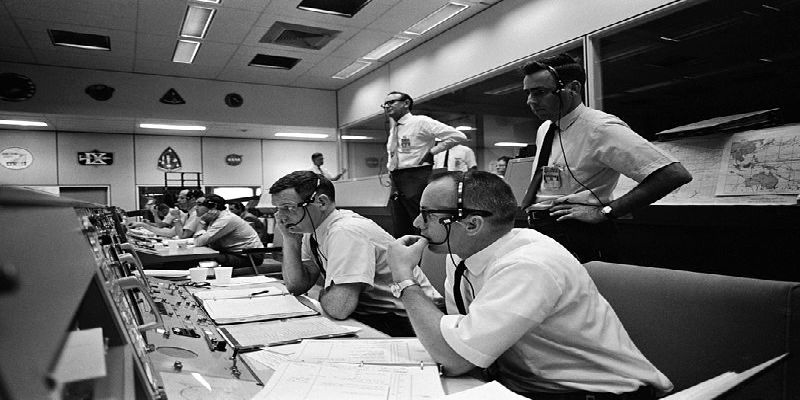
\includegraphics[height=2.0 in]{images/ATHENAsoc.jpg}
\caption{Monitoring centers }
\label{schema}
\end{center}
\end{figure} 
\section{Agile methodology: Kanban}

In this section, we introduce the working methodology adopted during the internship.
As a matter of fact, we chose to work with the agile Kanban to organize our tasks and
assignments.
\subsection{Definition}

Kanban is a lean method to manage and improve work across human systems. This
approach aims to manage work by balancing the demands with available capacity and improving the handling of system-level bottlenecks.

Work items are visualized to give participants a view of progress and process, from start
to finish usually via a Kanban board. Work is pulled as capacity permits, rather than work
being pushed into the process when requested. This provides a visual process management
system which aids decision-making about what, when and how much to produce.
\subsection{Characteristics}

The main characteristics of the adopted methodology are:
    \begin{itemize}
        \item Visualization: Creation of a board with post-it notes describing the tasks to perform
        and specifying their progress as illustrated on Figure \ref{kanban}.
        \item Limitation of the quantity of the work in progress: Split the list of tasks that would be endless into a series of reduced lists.
        \item Continuous Improvement: Ability to add new tasks whenever the capacity allows it.
    \end{itemize}
\begin{figure}[!htpb]
\begin{center}
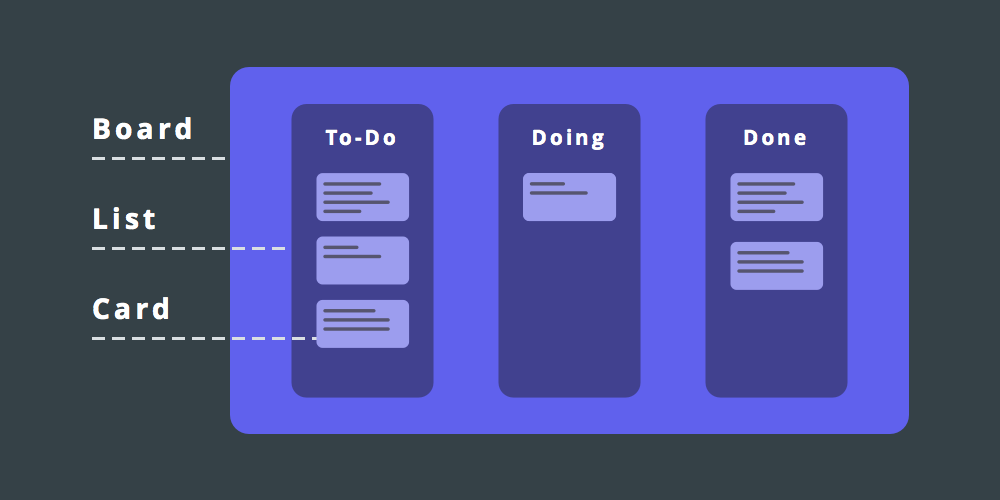
\includegraphics[height=3.0 in]{images/ATHENAkanban.png}
\caption{Illustration of a Kanban board}
\label{kanban}
\end{center}
\end{figure} 
\subsection *{Conclusion}

This chapter included a presentation of the hosting company, the context of the project and an overview of the problem settings. Moreover, we defined our agile methodology. The next chapter is devoted for the study
of the state of the art, the features that are already implemented and those that should be added in this project.


%------------------------------------------chapter2 Preliminary Study
\chapter{Preliminary Study}

\renewcommand{\chaptername}{Chapter}

In this chapter, we start by studying the state of the art and we present the most important concepts evoked in  our project. Then we study the existing solution by defining its efficiency and its imperfections. Afterwards, we present our own additional provision.



%----------------------------------------------State of the art
\section{State of the art}

To be able to develop our project, a state of art study is in order. It helps understand the frameworks surrounding the new technologies that will be used to accomplish this work.

We devote this part to explain IT terms as well as the architecture of an Network security monitoring toolkit along with a comparative study between different existent solutions. The IT terms include the technical terms we use throughout the application's realization.


\subsection{IT items}
In this part, we define the network security, monitoring, intrusion detection and preventions systems, honeypots, threats and threat intelligence.

\begin{itemize}[label=\ding{112}]

\item\textbf{Network security }

\begin{figure}[!htpb] 
\begin{center}
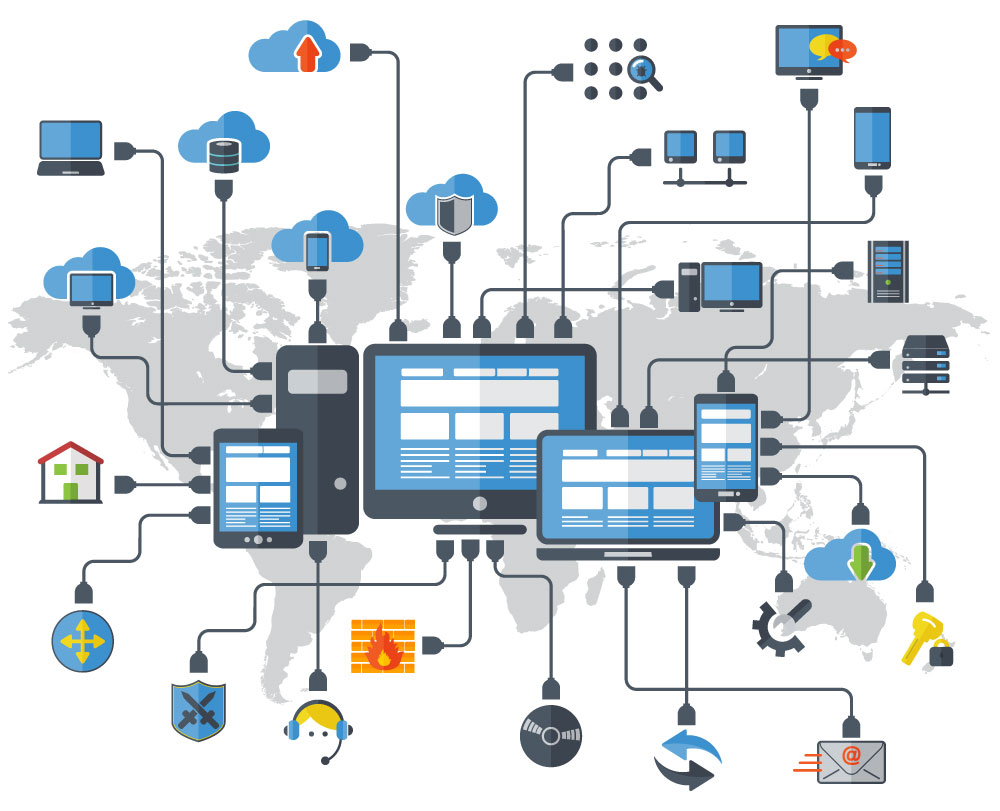
\includegraphics[height=3.6 in]{images/ATHENAnetsec.jpg}
\end{center}
\caption{ Network security }
\label{netsec}
\end{figure} 
As described in Figure \ref{netsec}, enterprises uses network to connect almost all of their components in each department or field finance, development, administration and sometimes from home or connected with clients, network is then critical as it guaranties access through equipment and personal data. Therefore, network security becomes a necessity because the control of access to files and directories is imperative against hacking, misuse and unauthorized changes to the system. Nowadays, some solutions may be integrated in companies like firewalls and anti-viruses, but is that really enough?  

\item\textbf{Monitoring}

Network monitoring can be many ways of recording traffic both ways inside the enterprise or outside the internet, those recordings changes format according to what product or solution is used. 
Even though some products controls access to enterprise's network, there is always a chance for attackers to gain access and bypass those implemented ways of protection, for that, monitoring network traffic in a company becomes useful to prevent breaches sometimes before it happens or later during investigation for it doesn't happen again. A couple of (free/payed) monitoring solutions is well known at the market like PRTG, NetworkMiner and other sniffers, but there is always a problem in those product either it is highly expensive or demands a lots of disk space and a group of analysts other than the community guidance that is often payed. 
\item\textbf{ IDS / IPS }

Intrusion Detection or prevention systems are network security appliances that monitor network or system activities for malicious activity. An Intrusion Detection System (IDS) is the process of monitoring the events occurring in your network and analyzing them for signs if possible incidents, violations or threatens your security policies. In the other hand Intrusion Prevention system is performing an IDS with the ability of stopping the detected incidents. IPS are often used because of the problems it may occurs to the enterprises for example stopping service(s) according to a false alarm(s). 
\begin{figure}[!htpb] 
\begin{center}
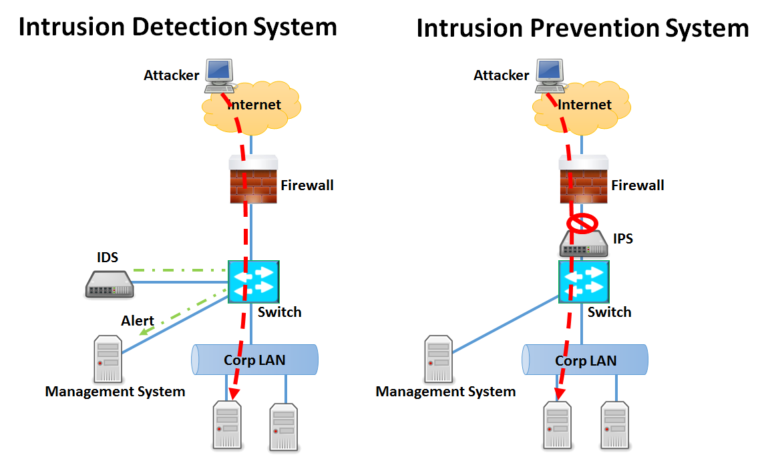
\includegraphics[height=3.6 in]{images/ATHENAidsips.png}
\end{center}
\caption{ IDS / IPS }
\label{idps}
\end{figure}


\item\textbf{Honeypots}

Honeypots are defined as decoy systems, their goal is to divert malicious traffic away from important systems, deployed alongside production systems with the intent of tricking hackers and gather information about intruders and guaranties early warning of a current attack before critical systems are hit. Those informations can be used for forensic or legal purposes.
\item\textbf{Threat intelligence}

In a military, business or security context, intelligence is information that provides an organization with decision support and possibly a strategic advantage. Threat intelligence is a component of security intelligence and includes both the information relevant to protecting an organization from external and inside threats as well as the processes, policies and tools designed to gather and analyze that information.
\end{itemize}
\subsection{Comparative analysis }
\subsubsection{ Intrusion Detection/Prevention Systems}
In the following comparison, three main point are compared (Performance, usage and Community)
\begin{itemize}[label=\ding{112}]
\item\textbf{Open-Source}

\begin{figure}[!htpb] 
\begin{center}
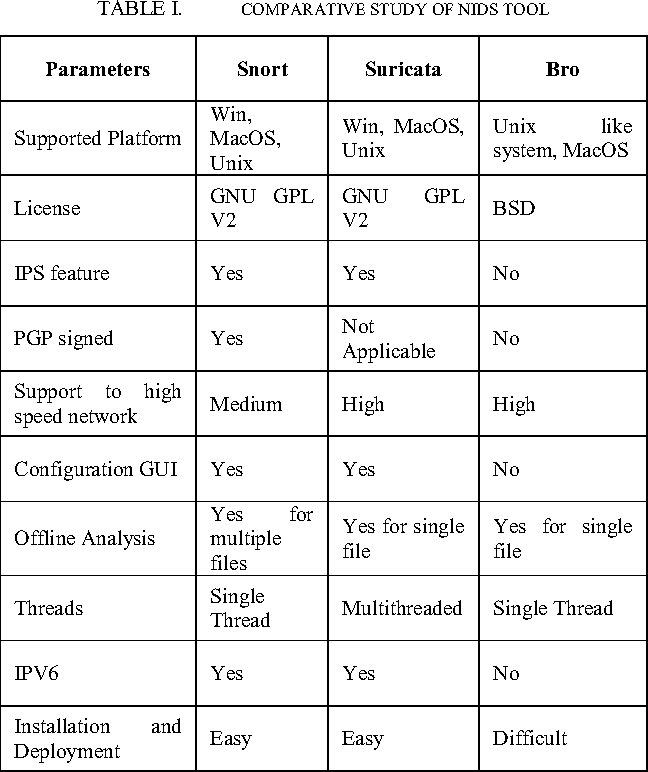
\includegraphics[height=3.8 in]{images/ATHENANIDS.png}
\end{center}
\caption{ Semantic Scholar Network IDS/IPS comparative analysis }
\label{nids}
\end{figure}
Snort , Suricata and Bro are the main three most powerful networks intrusion detection and/or prevention system in the world market. Based on the comparative analysis mentioned by Semantic scholar in Figure \ref{nids} and the test platform we performed : Snort is highly efficient in the scenario of moderate traffic with a single core processor. Based on architecture, snort uses 10 percent of CPU for parsing, 10 to 20 percent for normalization and 70 to 80 percent of CPU for payload inspection and detection. In a test performed by SANS, Snort gave a performance of 500Mbps with 1 CPU core for 1000 signatures. For 4000 signatures, it required 2.4 CPU at a rate of 400Mbps. It was found that a single instance of Snort is more efficient than Suricata with 50 percent less memory use. Recent versions of Snort support PF-RING and PCAP acceleration providing support for higher traffic. 

Suricata is more focused on large scale networks. In a way, it could be considered as an extension of Snort for large networks. In a scenario with a 45 CPU hosting 12 cores per CPU and 125 GB of RAM, the network throughput was 20 Gbps. Suricata had a very less packet drop of 7 percent while it was 53 percent in Snort. Suricata provides support for PF-Ring, AF packet, PCAP acceleration and NFLOG. It also works better with multi-threading. In snort the normalization is performed for every instance while for Suricata and Bro, the normalization is performed only once before multithreading. Suricata also support GPU cuda acceleration for pattern matching. There are also about 4000 file types build for file extraction and logging also providing MD5 matching. 

Bro as mentioned above is script driven IDS. Bro has support for clustering for high throughput environments. Bro provides a worker based architecture to use multiple processors. 
Bro’s developers recommend allocating one core for every 80 Mbps of traffic that is being analyzed.
It also have features allowing to interact with other systems in the enterprise, send email messages, page on-call staff, or automatically terminate existing connections. Bro also works based on file hash extraction and matching with the use of publicly available hash registers.
It is important to notice that the processing per core is significantly low compared to Snort or Suricata. But Bro has built in capacity to spread the load across multiple machines via Bro cluster thereby proving greater scalability. 
But there have some research showing that the overhead of distributed processing slows down the performance. Thus the performance acceleration is applicable only till a certain saturation point.

As for the usage, Suricata has a very similar rule set and configuration parameters to snort. While Bro could be called a behavior based one, with a very different approach compared to the idea of rules. Bro works with scripts. 

\begin{figure}[!htpb] 
\begin{center}

\includegraphics[height=1 in]{images/ATHENAnidss.png}
\end{center}
\caption{ Snort, Suricata and Bro logos }
\label{nidss}
\end{figure}

An IDS solution is only as good as the available rules it can apply to the monitored traffic. Snort has always had a lot of community support, and this has led to a substantial ruleset, updated on a regular basis. 

Suricata can use the same rules as SNORT. Many, but not all, VRT rules do still work. Suricata has its own ruleset, initially released to paying subscribers, but freely available after 30 to 60 days.

There is a number of resources available to provide help with using Bro, including channels to reach out the broader community and a commercial option for sites that need professional support.
\item\textbf{Paid Solutions}

Non Free products for intrusion detection or prevention systems are aften integrated with firewalls or Network Security Monitoring (NSM) tools, pre-configured by the provider and its support group for later charges in case of later modifications or re-configurations wanted by the client. An example of well known and trusted products are mentioned below:
\begin{itemize}
    \item Juniper Networks uses its SRX Series Services Gateways for intrusion detection and prevention (IDP) services. 

    \item McAfee uses its network threat and intrusion prevention solution Network Security Platform (NSP).
\end{itemize}

Since ATHENA is interested in new technologies and open-source products, while free open-source IDS and IPS software exists, these solutions often require an IT pro to make sure the IDS and IPS rules are up-to-date.

For a network such as ATHENA’s, it is more suitable to integrate Bro and Snort, as we can see with Bro’s great flexibility and Snort’s functionalities we can assume that nearly 100 percent of anomalies should be detected and reported.

\end{itemize}
\subsubsection{ SIEM }
\begin{figure}[!htpb] 
\begin{center}
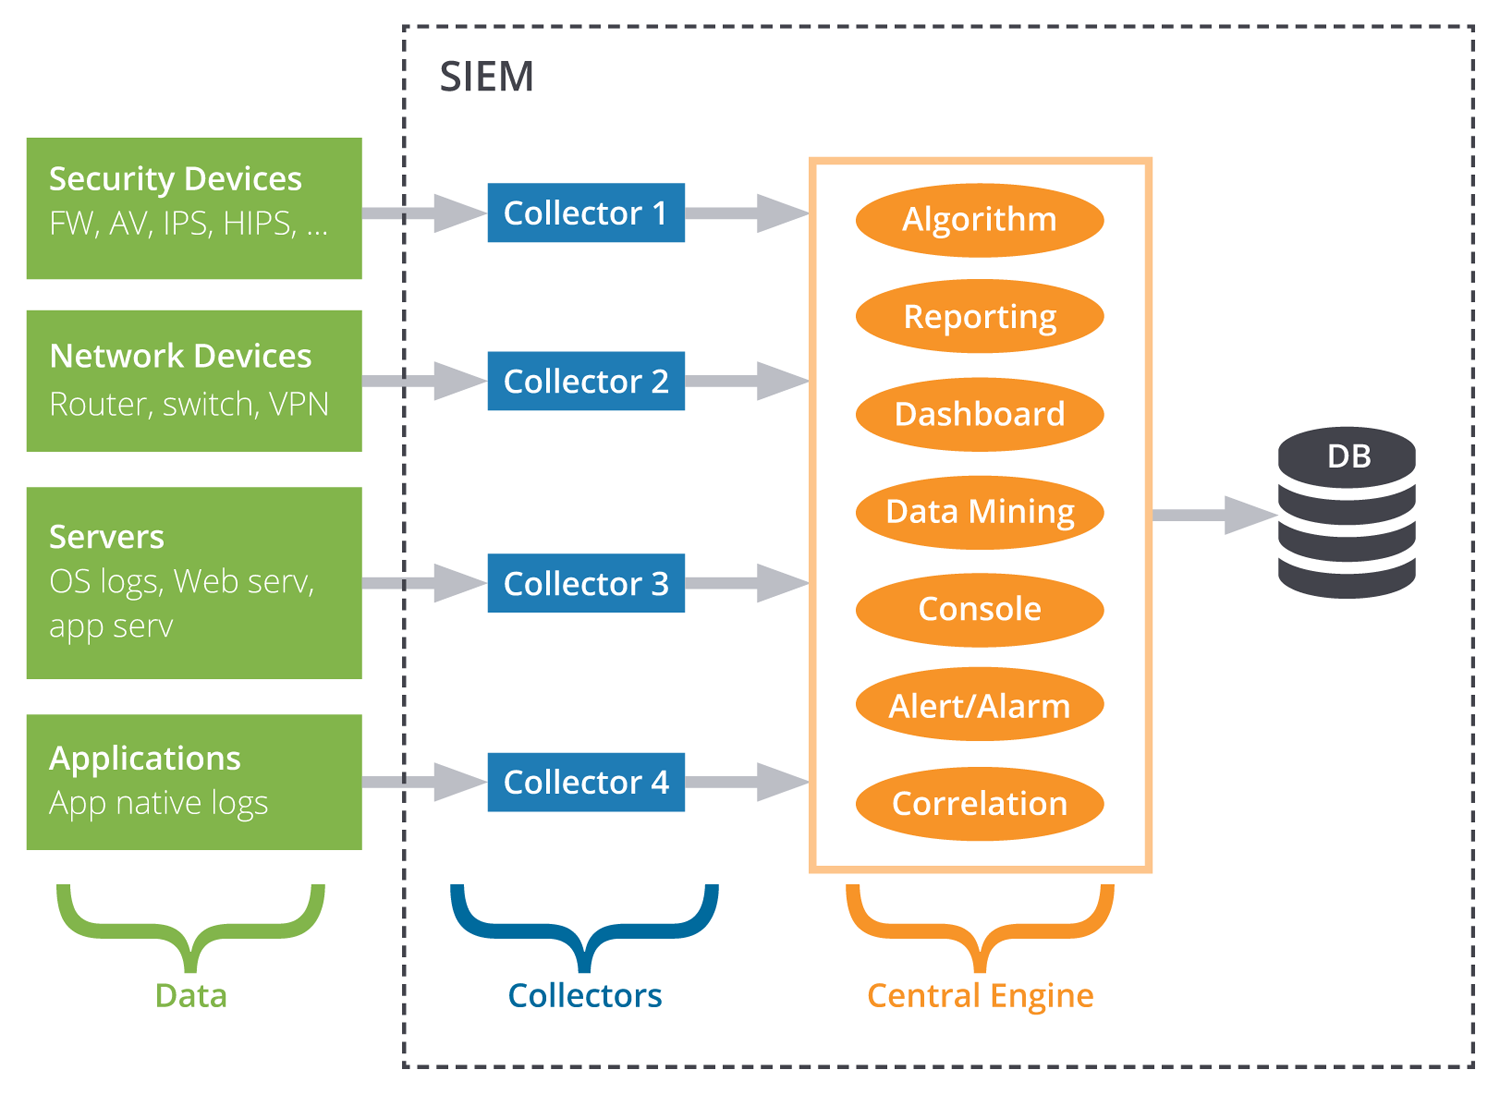
\includegraphics[height=3.0 in]{images/ATHENAsiem.png}
\end{center}
\caption{ Security information and event management }
\label{siem}
\end{figure}
Security information and event management (SIEM) is as mentioned in Figure \ref{siem}, a combination between security information management (SIM) and security event management (SEM). A centralized management platform of security events and alerts.
We focused on the the two main powerful solution in the world market according to test result of both solutions and user experience, Splunk and ELK :

\begin{itemize}
    \item ELK 
    
    It's a free open-source combination between ElasticSearch which is distributed, RESTful, JSON-based search engine. Easy to use, scalable and flexible. Logstash the powerful ingest pipeline and Kibana the flexible visualization tool. The Elastic Stack is loved by developers, From the perspective of the technical staff at Search Technologies, however, getting up to speed on ELK was relatively easy. They commented that the developer experience is also very good.
    \item Splunk
    
    Splunk Still Rules the Log Analytics Market for log analytics applications, and with over 500 million Dollars in revenues, Splunk is still the undisputed market leader. 
\begin{figure}[!htpb] 
\begin{center}
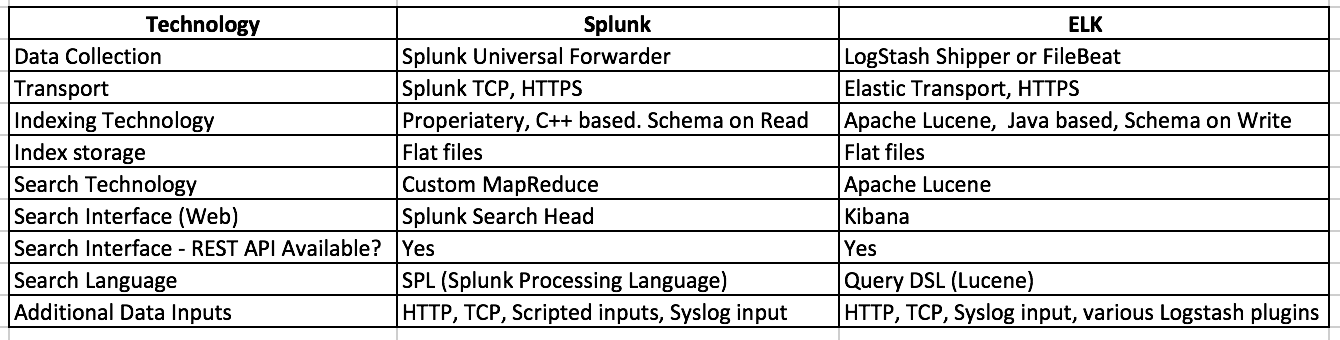
\includegraphics[width=18cm]{images/ATHENAsiemcompare.png}
\end{center}
\caption{ SIEM Comparative analysis }
\label{siemcomp}
\end{figure}

As in Figure \ref{siemcomp}, splunk and Elastic Stack are technically different.
In short, both Splunk and ELK/Elastic Stack are competent, enterprise-grade log management and analysis platforms trusted by the world's leading organizations. Total cost of ownership can be significant for both solutions; in response to demand from more budget-minded firms, Splunk and Elastic have recently started to offer hosted versions of their products. 

\end{itemize}
\subsubsection{ Security Monitoring Operating systems}

A network security monitoring toolkit has been always an interest to all enterprises, therefore some solutions already runs the market, in this section we are going to compare some of the most powerful security monitoring open-source solutions 

\begin{itemize}[label=\ding{112}]
\item\textbf{SELKS}

An Optimized hardware and multi layered Linux based operating system(both Live and installable Network Security Management ISO based on Debian) developed by Stamus Networks, the French company with headquarters in Paris who  believes in the innovative power and flexibility that Open Source Software posses. 
SELKS is combination of Suricata as its intrusion detection system, ELK as its SIEM and Scirius as a web management interface for Suricata rules and alerts, SELKS is currently running with a stable version 4.0 and as it shows in Figure \ref{selks}, it guaranties the following features :
\begin{itemize}
    \item Intrusion Detection System with ETPRO ruleset and your company/site/department specific rules.
    \item Web management interface: ruleset, config parameters.
    \item Log analysis via a scalable Elasticsearch with real time search and drill-down approach.
    \item Container: GNU/Linux distributions to run any task on Suricata generated data (IOC, connection to the SIEM).
    \item Network Security Monitoring: HTTP, DNS, TLS, SSH, File extraction, alert logging and many more.
    \item Proven 10+ Gbps full inspection.
    \item Enterprise support.
    \item Multi probe/Multi site scalable deployment.
\end{itemize}

\begin{figure}[!htpb] 
\begin{center}
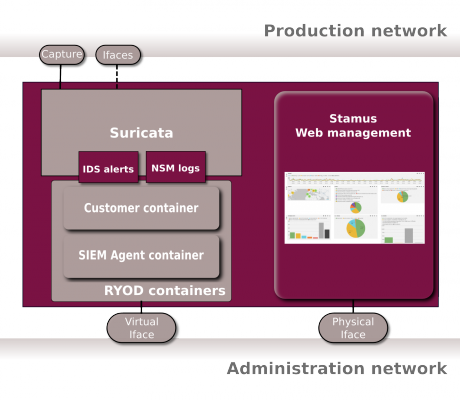
\includegraphics[height=3.6 in]{images/ATHENAselks.png}
\end{center}
\caption{ SELKS }
\label{selks}
\end{figure}

\item\textbf{SecurityOnion}

Security Onion is a free and open source Linux distribution maintained by Doug Burks  for intrusion detection, enterprise security monitoring, and log management. It includes Elasticsearch, Logstash, Kibana, Snort, Suricata, Bro, OSSEC, Sguil, Squert, NetworkMiner, and many other security tools. The easy-to-use Setup wizard allows you to build an army of distributed sensors for your enterprise. 

Security Onion seamlessly weaves together three core functions:
    \begin{itemize}
        \item Full packet capture.
        \item Network-based and host-based intrusion detection systems (NIDS and HIDS, respectively).
        \item and powerful analysis tools.
    \end{itemize}

Network-based and host-based intrusion detection systems (IDS) analyze network traffic or host systems, respectively, and provide log and alert data for detected events and activity. Security Onion provides multiple IDS options:
    \begin{itemize}
        \item\textbf{Rule-driven NIDS}
        
        For rule-driven network intrusion detection, Security Onion offers the choice of Snort or Suricata.
        \item\textbf{Analysis-driven NIDS}
        
        For analysis-driven network intrusion detection, Security Onion offers The Bro Network Security Monitor, also known as Bro IDS.
    \end{itemize}
For host-based intrusion detection, Security Onion offers OSSEC, a free, open source HIDS for Windows, Linux and Mac OS X. When you add the OSSEC agent to endpoints on your network, you gain invaluable visibility from endpoint to your network’s exit point. 
\begin{figure}[!htpb] 
\begin{center}
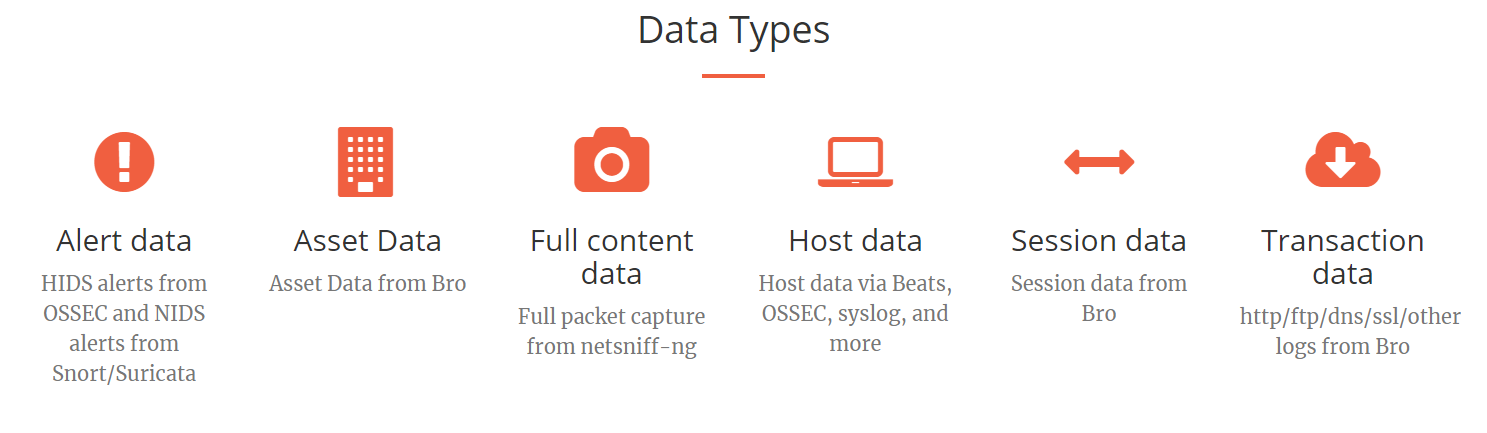
\includegraphics[width=18 cm]{images/ATHENAsoso.png}
\end{center}
\caption{ SecurityOnion Retrievable Data types }
\label{so}
\end{figure}
With full packet capture, IDS logs and Bro data, there is a daunting amount of data available at the analyst’s fingertips. Fortunately, Security Onion integrates the following tools to help make sense of this data:
    \begin{itemize}
        \item\textbf{Sguil} 
        
        Created by Bamm Visscher (@bammv), is “The Analyst Console for Network Security Monitoring.” It is the analyst’s right hand, providing visibility into the event data being collected and the context to validate the detection. Sguil provides a single GUI (written in tcl/tk) in which to view Snort or Suricata alerts, OSSEC alerts, Bro HTTP events, and Passive Real-Time Asset Detection System (PRADS) alerts. More importantly, Sguil allows you to “pivot” directly from an alert into a packet capture (via Wireshark or NetworkMiner) or a transcript of the full session that triggered the alert.
        
        \item\textbf{Squert}
        
        Created by Paul Halliday (@01110000), is a web application interface to the Sguil database. Although it is neither meant to be a real-time (or near real-time) interface nor a replacement for Sguil, it allows querying of the Sguil database and provides several visualization options for the data such as “time series representations, weighted and logically grouped result sets” and geo-IP mapping.
\end{itemize}


Security Onion is built on a distributed client-server model. A Security Onion “sensor” is the client and a Security Onion “server” is, well, the server. The server and sensor components can be run on a single physical machine or virtual machine, or multiple sensors can be distributed throughout an infrastructure and configured to report back to a designated server. An analyst connects to the server from a client workstation (typically a Security Onion virtual machine installation) to execute queries and retrieve data.
The following are the three Security Onion deployment scenarios:
    \begin{itemize}
    \item\textbf{Standalone:}
    
    A standalone installation consists of a single physical or virtual machine running both the server and sensor components and related processes. 
    \item\textbf{Server-sensor:}
    
    A server-sensor installation consists of a single machine running the server component with one or more separate machines running the sensor component and reporting back to the server.
    \item\textbf{Hybrid:}
    
    A hybrid installation consists of a standalone installation that also has one or more separate sensors reporting back to the server component of the standalone machine.
    \end{itemize}

\end{itemize}


%%%%%%%%%%%%%%%%%%%%%%%%%%%%%%%%%%%%%%%%%%%%%%%%%%%%%%%%%%%%%%%%%%%%%%%
%%%%%%%%%%%%%%%%%%%%%%%%%%%%%%%%%%%%%%%%%%%%%%%%%%%%%%%%%%%%%%%
\ifx
SaaS cloud level is usually a catalog of applications available as a service to end users or customers.
In other words, this level offers a range of services "modable" and "customizable". It may be noted as an example a courier, CMS, access to libraries, shopping in online stores etc.
Using this mode is also useful when prototyping phase in a short time and at low cost.

Cloud service models Cloud Computing as general term sits over a variety of services
from Infrastructure as a Service at the base, through Platform as a Service as a development
tool and through to Software as a Service replacing on-premise applications.

Software as a Service (SaaS): SaaS is the highest level. At this level, the capability
provided to the consumer is to use the provider’s applications running on a cloud infrastructure.
The applications are accessible from various client devices through either
a thin client interface, such as a web browser (e.g., web-based email), or a program interface.
The consumer does not manage or control the underlying cloud infrastructure including network, servers, operating systems, storage, or even individual application capabilities, with the possible exception of limited user-specific application configuration settings.[B1]

\item\textbf{SPA }

A Single Page Application is a web developed application that can be displayed on a single web page in order to simulate the desktop application experience for users.
As the developers see it fit, it can either retrieve the necessary source code with one single page load, or dynamically load the necessary resources in response to the user requirements. The page in question does not reload at any point of the process nor modulate the data communication with other pages.


\item\textbf{Google Maps API }

Google provides many special-purpose APIs. The use of this specific API is mandatory while building a geolocalization application.
This part highlights the capability of Google map API.

It is a Google Application Programming Interface that handles the geolocalization of an address granted its latitude and longitude and spotting it on the map.
The Api provides multiple services such as mapping data display which offers Internet users a global geographic data vision. 

The data displayed on the map is dressed up as a pictogram: small clickable items. Once clicked, the icon leads to a set of information concerning the geolocalized data. 
It is also possible to set an itinerary by assigning the starting point and the destination which would generate a time estimation for each proposed itinerary.
It is also possible to calculate a route (pedestrian or car) from a starting point  to a point of arrival.[B2]
\fi


\ifx
\subsection{AJAX }
Ajax is a set of programming techniques or a particular approach to web programming. 
These programming techniques involve being able to seamlessly update a web page or a section of a web application with input from the server, but without the need for an immediate page refresh. This does not mean that the browser does not make a connection to the web server.

\begin{figure}[!htpb] 
\begin{center}
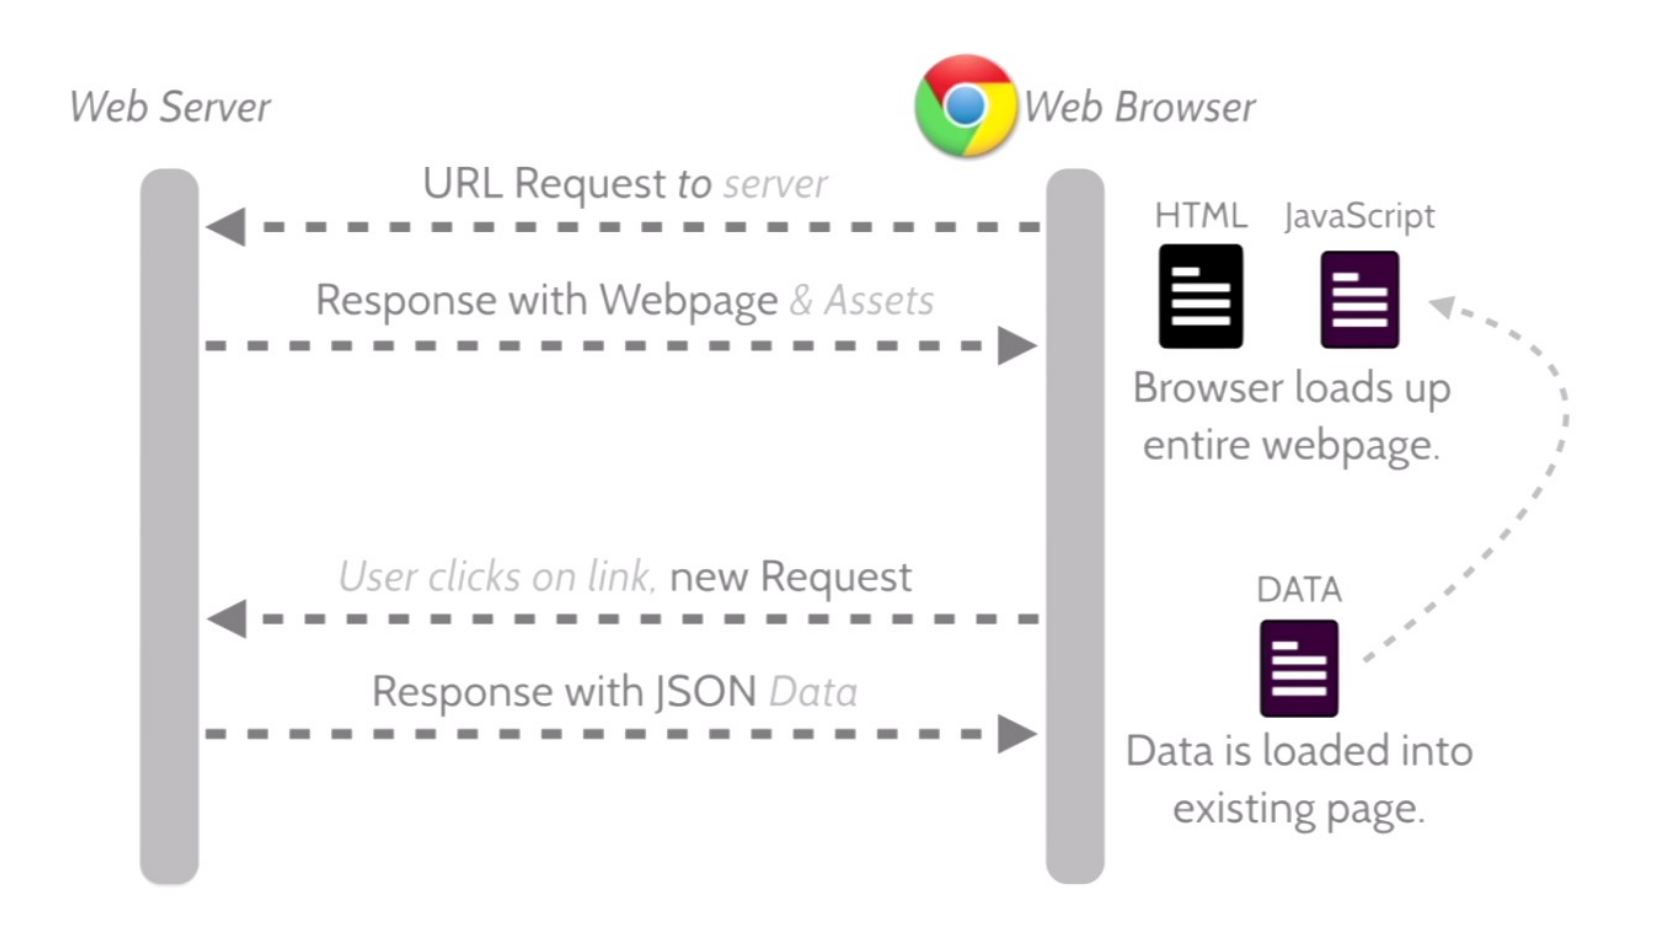
\includegraphics[height=3.6 in]{images/ajax2.png}
\end{center}
\caption{« AJAX » application }
\label{ajax}
\end{figure} 

Figure \ref{ajax} [B3] demonstrates how AJAX works. It allows web pages to be updated
asynchronously by exchanging small amounts of data with the server behind the scenes. This means that it is possible to update parts of a web page, without reloading the whole page. 
Classic web pages, (which do not use AJAX) must reload the entire page if the content should change. Examples of applications using AJAX: Google Maps, Gmail, Youtube, and Facebook tabs.
We explain and enumerate which technologies related to AJAX are incorporated in
the development of our application:

\begin{itemize}
    
    \item HTML (or XHTML) and CSS for presentation (to mark up and style the data).
    
    \item The HTML DOM defines a standard set of objects for HTML, and a standard way to access
and manipulate HTML documents. The utility of DOM is that all HTML elements, along with
their containing text and attributes, can be accessed through it. Their contents can be modified or deleted, and new elements can be created. DOM can be used by any programming language like
Java, JavaScript, and VBScript \cite{w3school}. In our Case we used it especially to manipulate the elements of the user interface.
Document Object Model (DOM) is accessed with JavaScript for dynamic display and
interaction with data. 


\item JSON is designed to be a data interchange format which is human readable and easy for computers to parse and use. JSON is directly supported inside JavaScript and is best suited for JS applications; thus providing significant performance gains over XML, which requires extra libraries to retrieve data from Document Object Model (DOM) objects. JSON is estimated to parse up to one hundred times faster than XML in modern browsers.Validation of inputs is the responsibility of individual domain applications, and the lack of extensibility claims is addressed by the flexibility of JSON constructs. \cite{json} The next lines describe an example of JSON to clarify its structure.

\{ "firstname" : "John",

"lastname" : "Smith" \}

\item JavaScript to bring these technologies together.

\end{itemize}
\fi %%%%%%%%%%%%%%%%%%%%%%%%%%%%%%%%%%%%%%%%%%%%%%%%%%%%%%%%%%%%%%%%% %%%%%%%%%%%%%%%%%%%%%%%%%%%%%%%%%%%%%%%%%%%%%%%%%%%%%%%%%%%%%%%

%--------------------------------------------------Study of existing and critics  & proposed solution


\section{Study of the solution}
~~~In this part, we describe briefly the solution already implemented and criticize its drawbacks. After that, we present the advantages of our proposed component.

As evoked in the previous chapter, the solution is a network security monitoring toolkit that offers services to complete a security operation center.

\subsection{ATHENA's network}

As the number of servers and services increases, it is becoming more and more challenging to control and observe the traffic passing by them all. Figure \ref{networkarch} exhibit the network architecture of ATHENA. 

~

\begin{figure}[!htpb]
\begin{center}
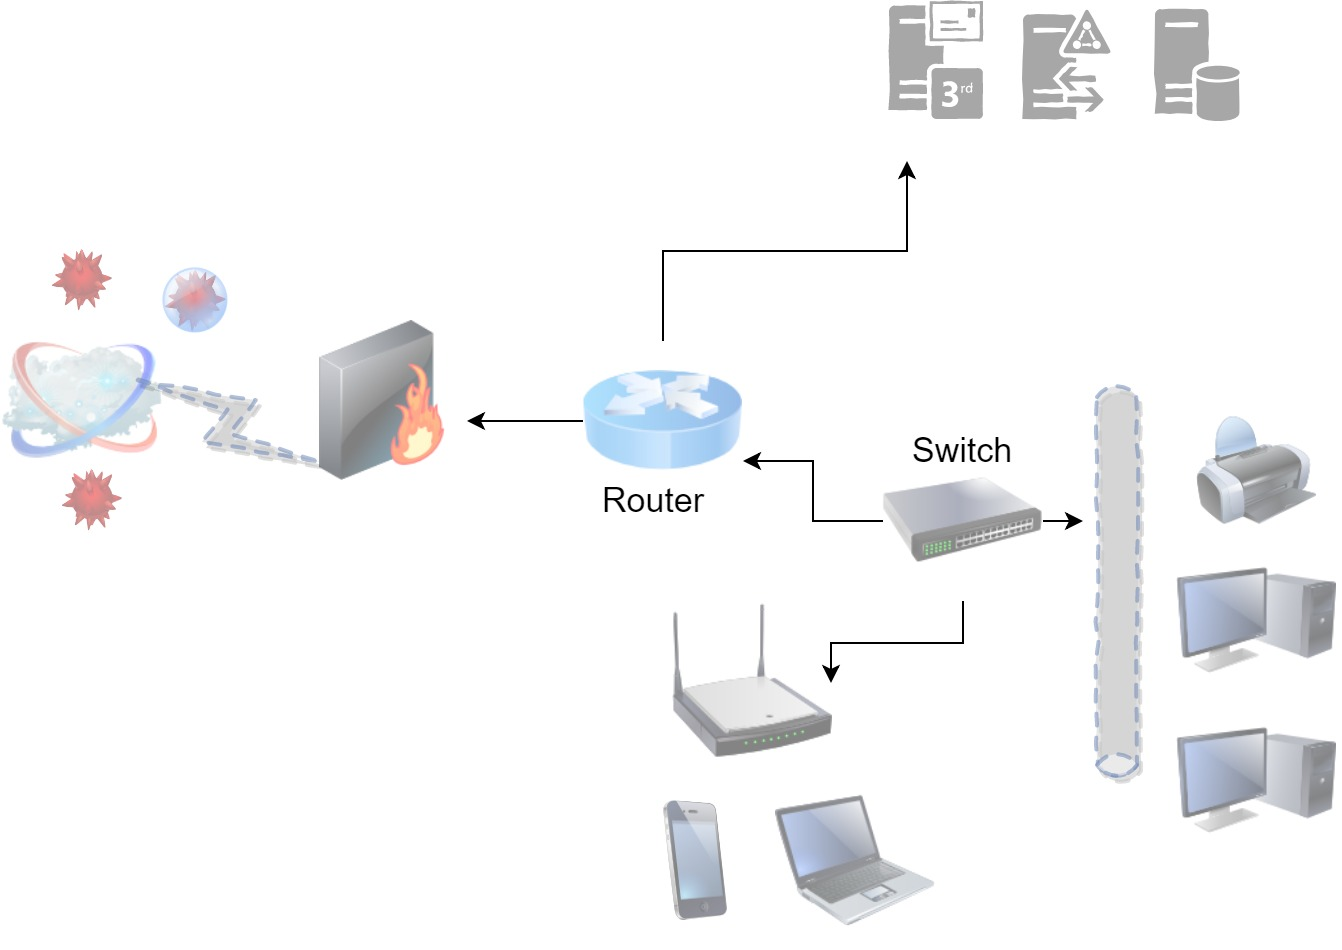
\includegraphics[height=3.5 in]{images/ATHENAnetw.jpg}
\caption{ATHENA's Network general view}
\label{networkarch}
\end{center}
\end{figure} 

Server are placed separately from the private network for security reasons, the private network is divided between physical and wireless connections, user's permissions are managed through vlans. An ASA firewall is well configured to prevent and control access from the outside.
\subsection{Proposed solution}

Based on the previous state of network in ATHENA, The major features of our solution should be:

\begin{itemize}
    \item Sensor or probe to monitor the traffic coming in and out both private and demilitarized zone.
    \item Incident response mechanism to report alerts.
    \item Visualization platform for analysts.
    \item Threat intelligence platform.
    \item Honeynet (Centralized management of Honeypots) to trick attackers and gather information about intruders.
    \item Servers and services monitoring.
    \item Management interface for analysts to control and deploy sensors.
\end{itemize}


~





%---------------------------------------------------------conclusion
\subsection *{Conclusion}
In this chapter, we went through a brief study of the state of the art while presenting the most important concepts used in this project. After that, we reviewed the existing solution and we highlighted our contribution.
In the next chapter, we enumerate the different features offered by our application and we present the main possible scenarios.



%--------------------------------------chapter3 Requirements Analysis and Specification 

\chapter{Requirements Analysis and Specification}
\renewcommand{\chaptername}{Chapter}

This chapter is dedicated to presenting and analyzing our project in a formal way. We specify the functional and non-functional requirements of our project. We then list the actors of our component along with their granted permissions. Finally, we formalize the identified features with the help of Use Case diagrams and we show the project's principal scenarios using system sequence diagrams.

\section{Requirement Analysis}

Throughout this section, we identify and present the different functional and non-functional requirements that our application should satisfy. 

\subsection{Functional Requirements}

Functional requirements refer to primary functions that the solution must fulfill once developed. The network security monitoring toolkit has to provide a specific set of services which are : 

\begin{itemize}[label={$\checkmark$}]

\item \textbf{Network traffic monitoring} 

The implemented probe should be able to collect all the traffic along with the correlated alerts and display them to the analysts. Probes should be configured to filter some traffic and a log rotation process to keep the probe's best performance.


\item \textbf{Servers and services monitoring} 

Our component must enable the analyst to know whenever a shutdown of services or servers is in place, also it may allow us to decide modifying hardware according to usage of resources.

\item \textbf{Visualization dashboards } 

The solution must enable the user (analyst) to search for threats or IOCs (indicators of compromise). It also allows him to view the corresponding event on the map. Also the ability to create dashboards to fit the needs of the analyst. 

\item \textbf{Threat intelligence platform} 

The system should be able to hunt down network threats before it even happens and see what others (Antivirus and IDS) can't detect.

\item \textbf{Management interface for probes} 

The management of probes should be done from a centralized interface. Rules should be tuned and filtered to respond to analyst's needs to cover all services. 

\end{itemize}

\subsection{Non-Functional Requirements}

Non-functional requirements refer to several key features that are beyond the purpose of the solution, they don't describe specific behaviors. Rather, these specific criteria ensure user's satisfaction and contentment.

\begin{itemize}[label={$\checkmark$}]

%------------------------BNF1
\item \textbf{Extensibility} 

The system must be able to allow and accept significant extension of its capabilities without major reconfiguration or changes in its basic architecture.

%------------------------BNF2
\item \textbf{Security} 

The system should be able to counter most of known vulnerabilities.

%------------------------BNF3
\item \textbf{Reliability and Viability} 

The system must function without a potential breakdown. In case of any failure, it must not corrupt any data or information that is already stored.


%------------------------BNF4
\item \textbf{Ergonomy} 

The implemented solution should provide a friendly user interface with clear components. This is possible by offering various options such as modifying the color, the size and the positions of the tabs. 


%------------------------BNF5
\item \textbf{Performance } 

The system should be as efficient as possible, and run without any potential breakdown. The analyst should be able to receive the final evaluation and result within a reasonable amount of time. 


\item \textbf{Re-usability }

Development and configuration for this solution is re-usable and may be used afterwards by others. It must be save as a template in order to be effective.

\item \textbf{Authorization levels } 

The system allows to control the privileges of individual users.
\end{itemize}


%-------------------------------------
\section {Requirement Specification}
~~On one hand, this section offers a better understanding of the mentioned requirements by declaring them in a semi-formal way.
On the other hand, it emphasizes the interactions between the actor and our toolkit. In contemplation of breaking down the complexity of these goals, we use the Use Case Diagrams.

%------------------------------------------------Actors
\subsection {Identification of the actors}
An actor is an abstraction of a role of actual user who is in a perpetual interaction with the toolkit. Following on, our system's actor along with his role and granted permissions.


\begin{itemize}[label={$\checkmark$}]
\item \textbf { Security analyst } 

He is the primary user of the system. His role is to maintain the security by monitoring and analyzing security events. He is granted privileges to access the threat intelligence platform so he can share his discoveries with the rest of security analysts.
\item \textbf { SOC manager }

He possesses all the privileges of a threat hunter, he can also manage users on the system and validate the suggested incidents.
\item \textbf { SIEM }

The SIEM is responsible for data centralization and provides query results and dashboards to the users(analysts).
\item \textbf { Probes }

The Probes are responsible for logs collection and correlation of different type of data and forward those logs to the SIEM.
\end{itemize}

%-----------------------------------------------UML
\subsection {Use Case Diagrams}

Figure \ref{usecase} describes the Use Case diagram, displayed from the main actor's perspective.


\begin{figure}[htbp!]
\begin{center}
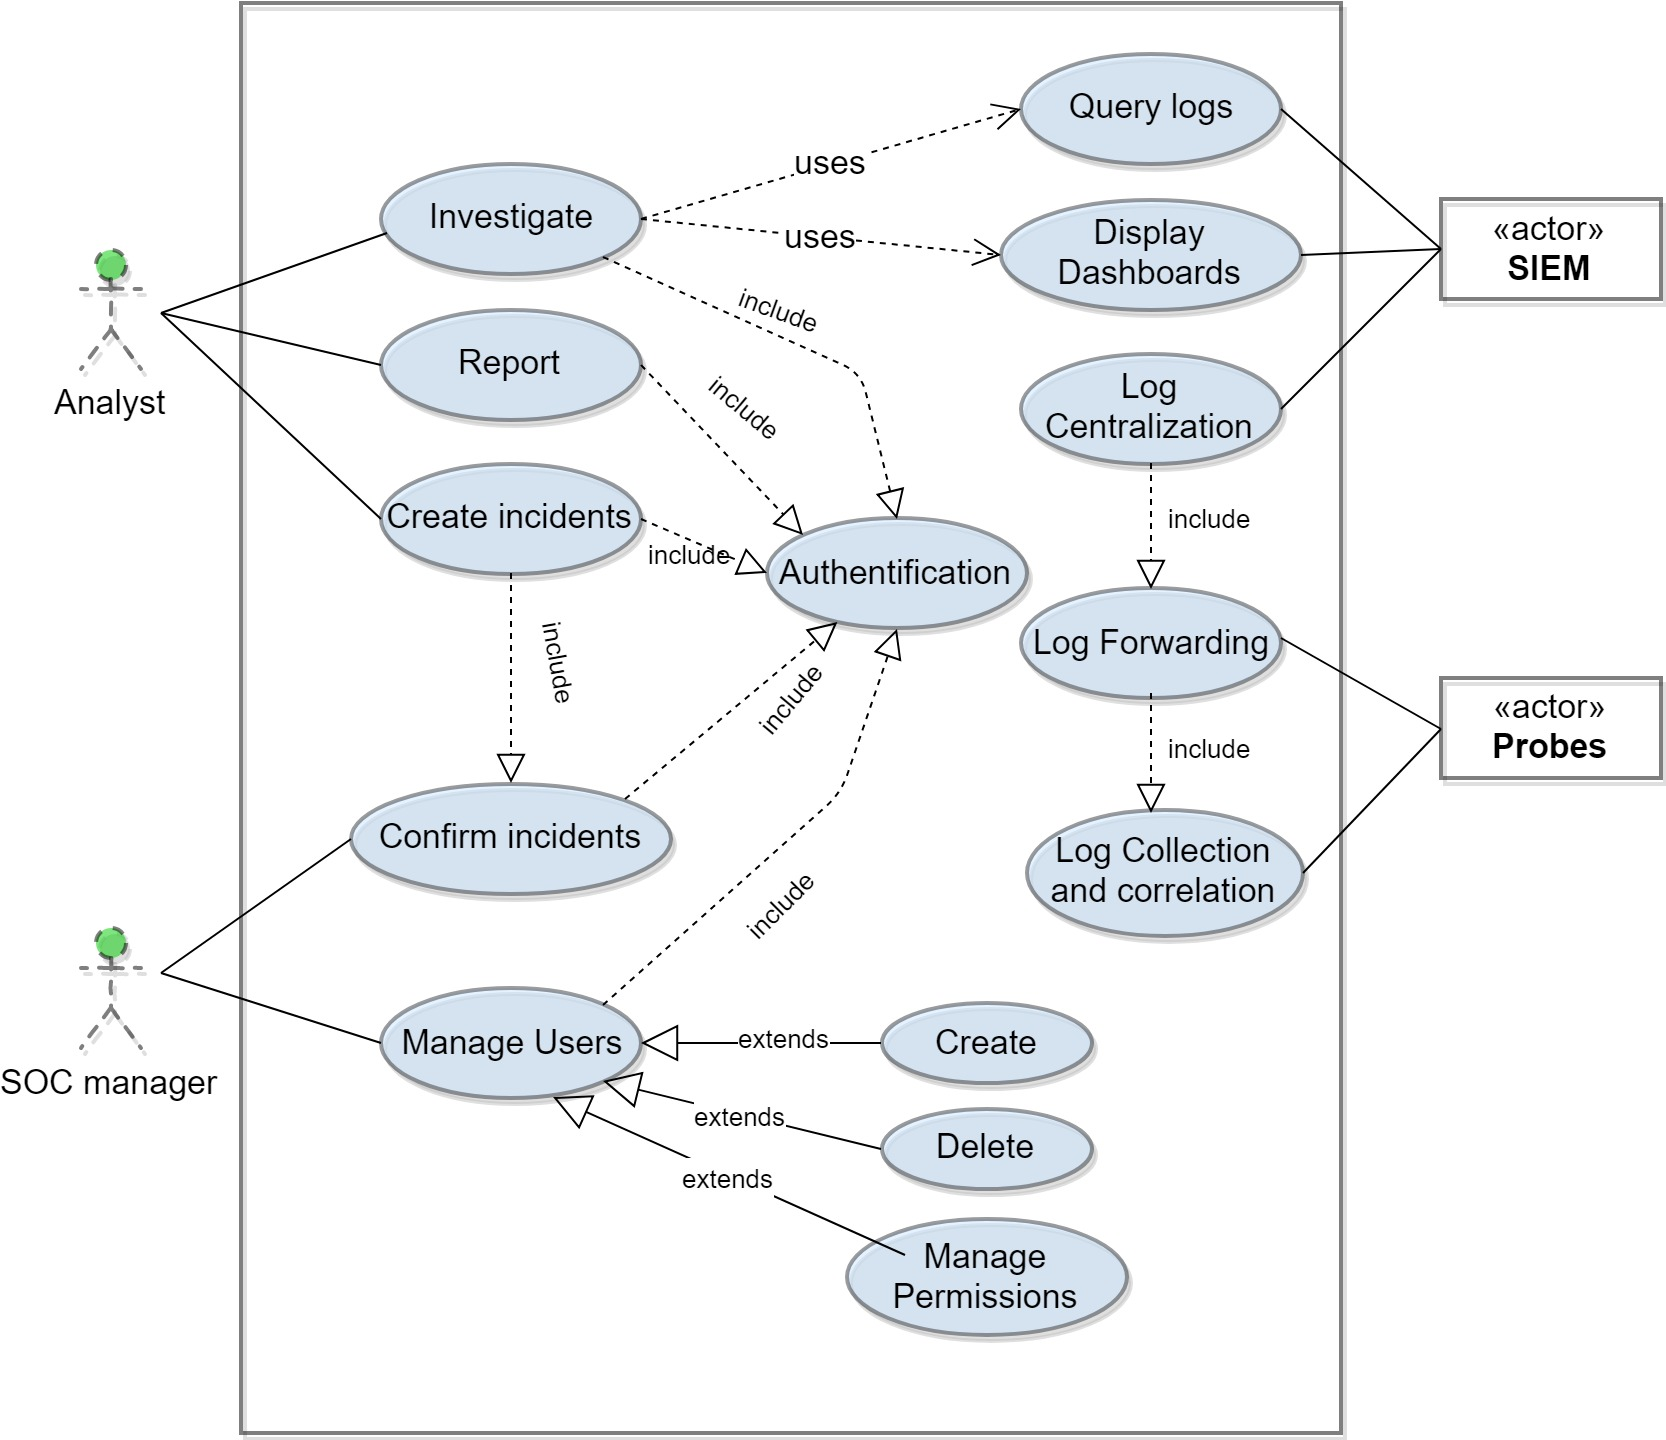
\includegraphics[width=5.5 in]{images/ATHENAusecaseDiagram.jpg}
\caption{System’s General Use Case}
\label{usecase}
\end{center}
\end{figure}  ~

\newpage

The analyst is able to view all logs and alerts through dashboards, the investigation process is accomplished via searching event and querying logs. 
A report must be created by the analyst depending on investigations then he can create incidents if there is an incident by its priority and wait for the SOC manager to confirm that incident.
The Soc manager can also manage users (analysts) and their permissions (which logs or platform to access).

The SIEM (Security information management system) plays a very important role in the system since it is responsible for log's centralization, display and must be efficient and guarantee information's availability and integrity whenever the analyst wants to query logs (old and real-time).

Probes are the main actor that is responsible for collecting and recording logs based on a list of predefined rules and scripts, correlate events and forward logs to the SIEM to prevent disk draining and system failure.

\subsection{Global Sequence Diagram}

In this section, we present the most relevant nominal scenarios in our application using the system sequence diagrams. In a brief description, each system sequence diagram considers one use case at a time and gives the sequence of actions between the user and the system.

\subsubsection *{Nominal scenario for 'Investigation' }

This scenario is illustrated by Figure \ref{seq_diag1}.

In order to start, the authenticated analyst demands summaries for events and alerts in dashboards. The system responds by loading the page, showing multiple dashboards in table, circles, lines and maps. The analyst has the option to filter those dashboards according to different criteria(time, IP address, host name or country name, protocol, port, etc.). 

As a response, the system displays the filtered dashboard. Then, if the analyst notices a malicious activity or a sequence of alerts, he must dug deeper in the details and in some cases extract the PCAP file (A capture file saved in the format that libpcap and WinPcap use can be read by applications that understand that format, such as tcpdump, and in our case Wireshark and NetworkMiner which comes with SecurityOnion) for later examination or proof of breach (for legal use). 

The analyst then creates a report about the incident. In order to do that, he can (if he has permission) access to the treat intelligence platform to see if bro logs indicates or confirm the incident. 

According to its priority, the analyst must create a detailed incident and send it to the SOC manager for confirmation.


\begin{figure}[htbp!]
\begin{center}
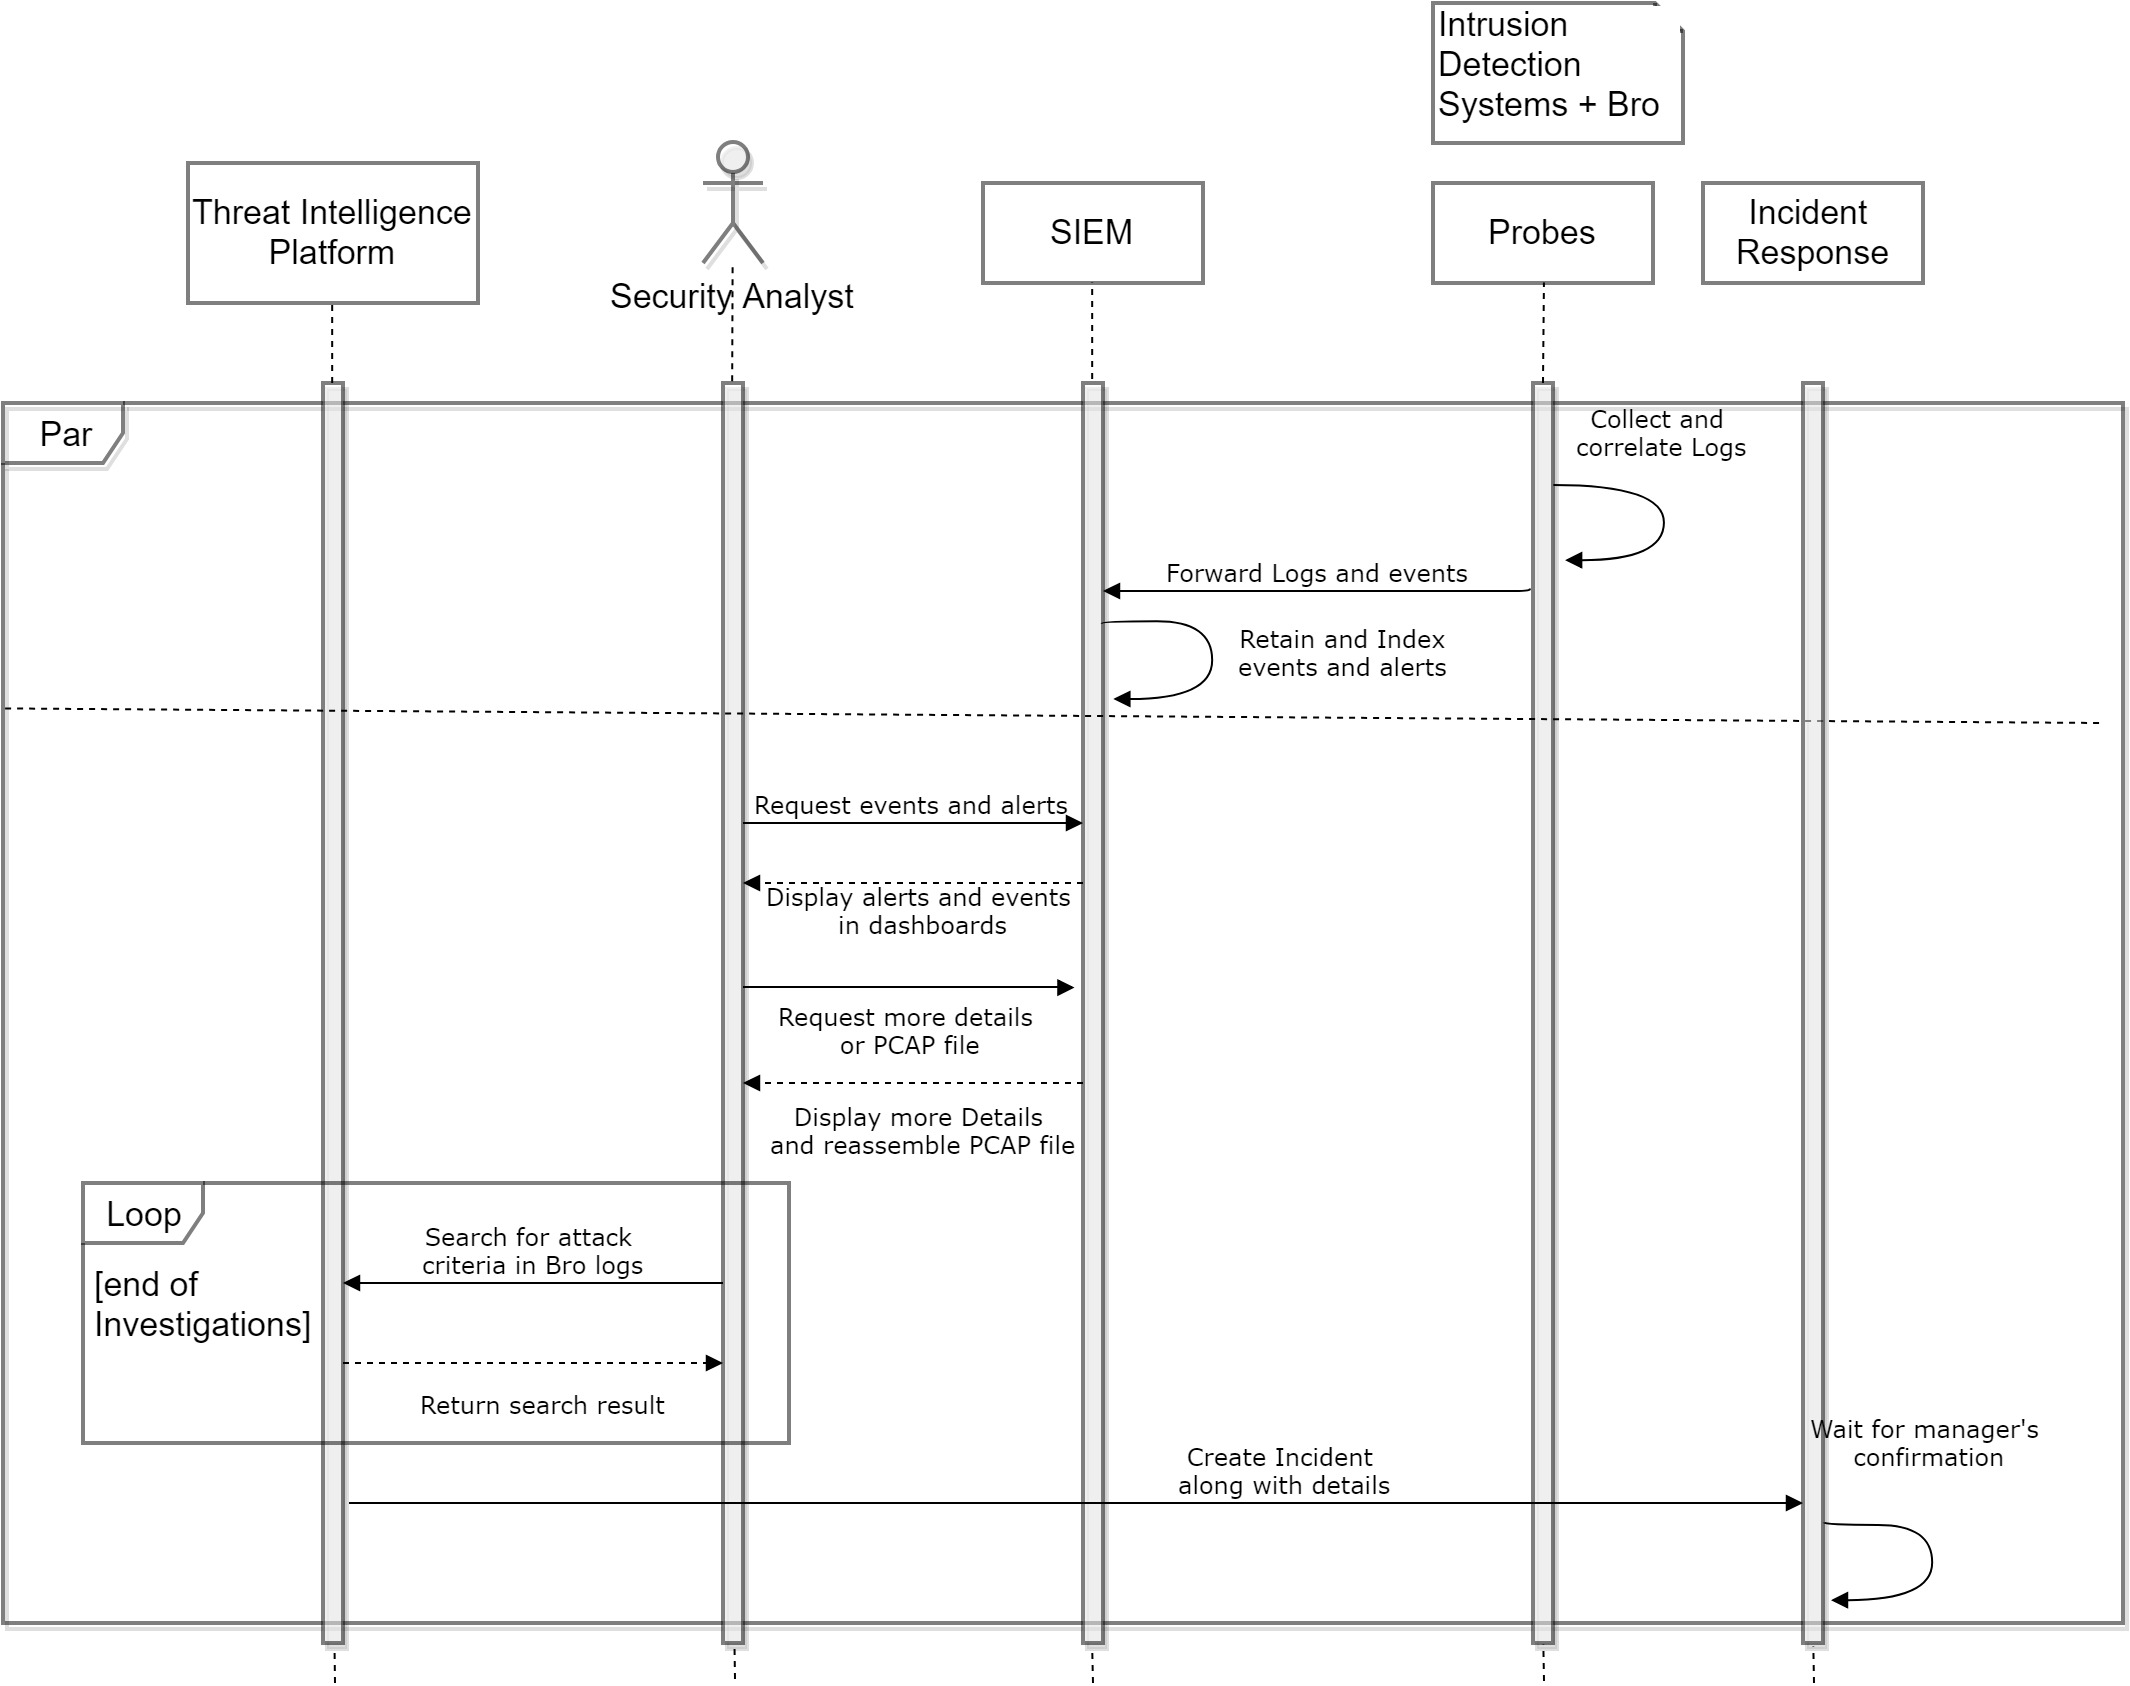
\includegraphics[height=5.0 in]{images/ATHENAGeneralseq.jpg}
\caption{’Investigation’ nominal sequence diagram}
\label{seq_diag1}
\end{center}
\end{figure} 


\subsubsection* {Nominal scenario for 'Incident creation'}

~~~This scenario is illustrated by Figure \ref{seq_diag2}.

The analyst is supposed to run an analyze on bro logs to detect if there is a malicious behaviour or attacks that are undetectable by anti-virus, firewall and even the regular intrusion detection system.

The analyst should have access to the based on local events threat intelligence platform, chooses the time-line(time interval) on which he wishes to run the analyze, the threat intelligence platform then pulls logs and events from the SIEM and index them to fit the pre-configured functions. then display the result in a web page in graphs and tables format. 

Based on those results, the analyst should create the incident report related to that time-line.


\begin{figure}[htbp!]
\begin{center}
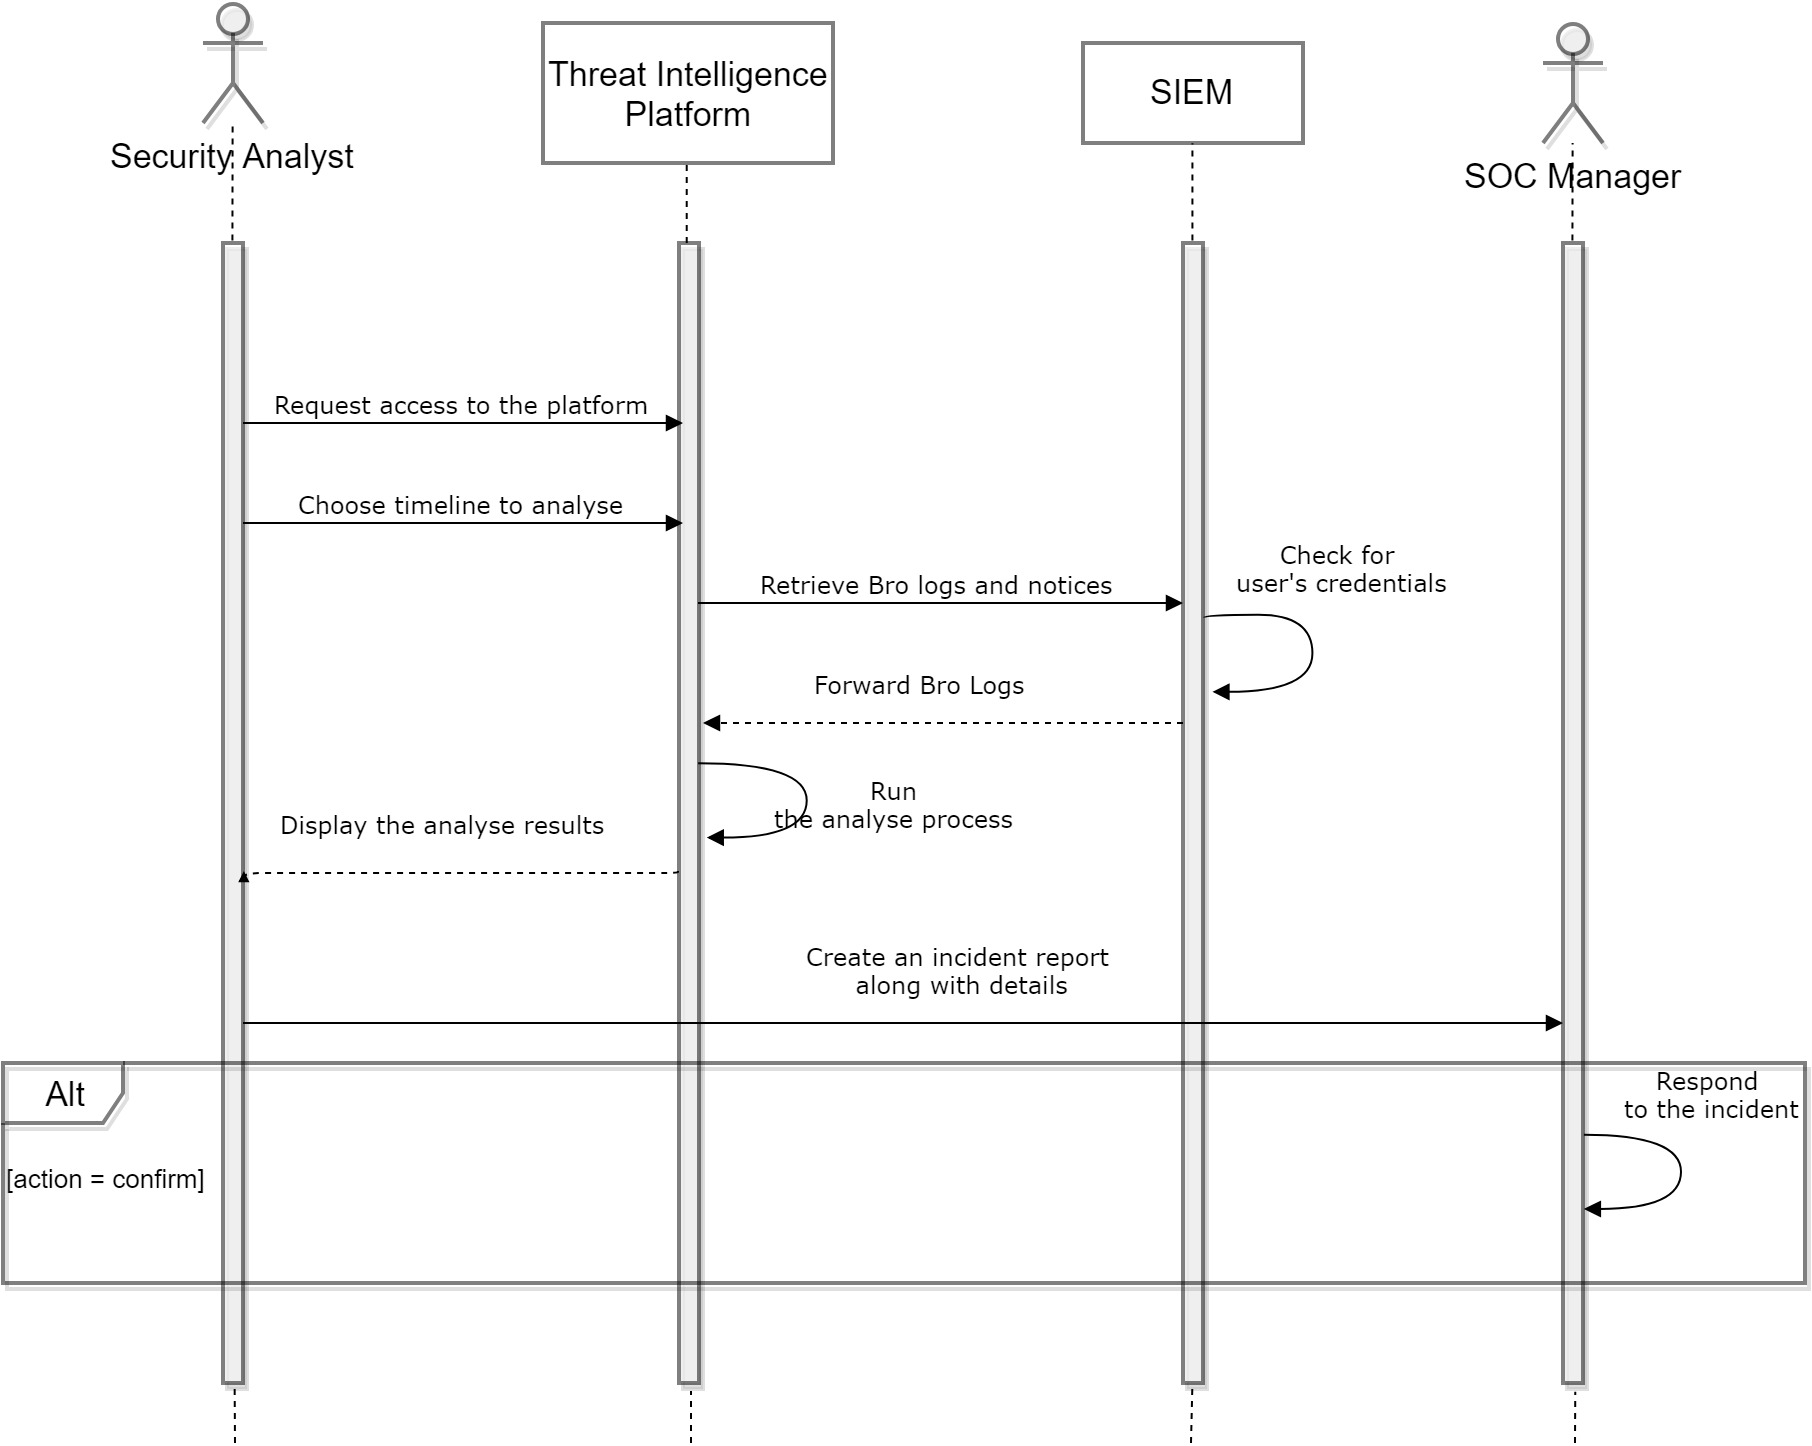
\includegraphics[height=5.0 in]{images/ATHENAThreatintel.jpg}
\caption{’Incident creation’ nominal sequence diagram}
\label{seq_diag2}
\end{center}
\end{figure} 


\subsection *{Conclusion}

Throughout this chapter, we specified and analyzed the requirements that our application should deliver to the future analysts, and we gave the main scenarios and Use Cases of our project. The next chapter aims to go a step further in the process of developing the application via presenting the application’s design.





%------------------------------------------chapter4 Design

\chapter{Design}
\renewcommand{\chaptername}{Chapter}


~~~~~In order to reach the appropriate result as described in the specifications, we need to clarify the
project main architecture, as well as the architecture of its components.

This chapter focuses on designing a suitable structure for the application. This step is crucial in the course of the project and aims to undertake and prepare the ground for the implementation phase.

\section{Physical architecture}
In this section, we briefly study the proposed architecture to make sure it is corresponding to the goals of the project.

Figure \ref{physic_arch} presents the physical architecture of our solution in ATHENA's network. In the following paragraphs, we describe each component of the architecture and the corresponding role.

\begin{itemize}
    \item \textbf{RITA:}
    
    Real Threat Intelligence Analysis is used as our threat intelligence platform, pulling Bro logs from our SecurityOnion Box for later analysis.
    \item\textbf{SecurityOnion Standalone box:} 
    
    This box is an instance of SecurityOnion along with its tools to sniff ATHENA's in and out traffic and run it through Intrusion Detection Systems(Suricata and Bro), correlate events and alerts for later use. It is connected directly to the switch with a port mirroring option(used on a network switch to send a copy of network packets seen on one switch ports).
    \begin{figure}[!htpb] 
    \begin{center}
    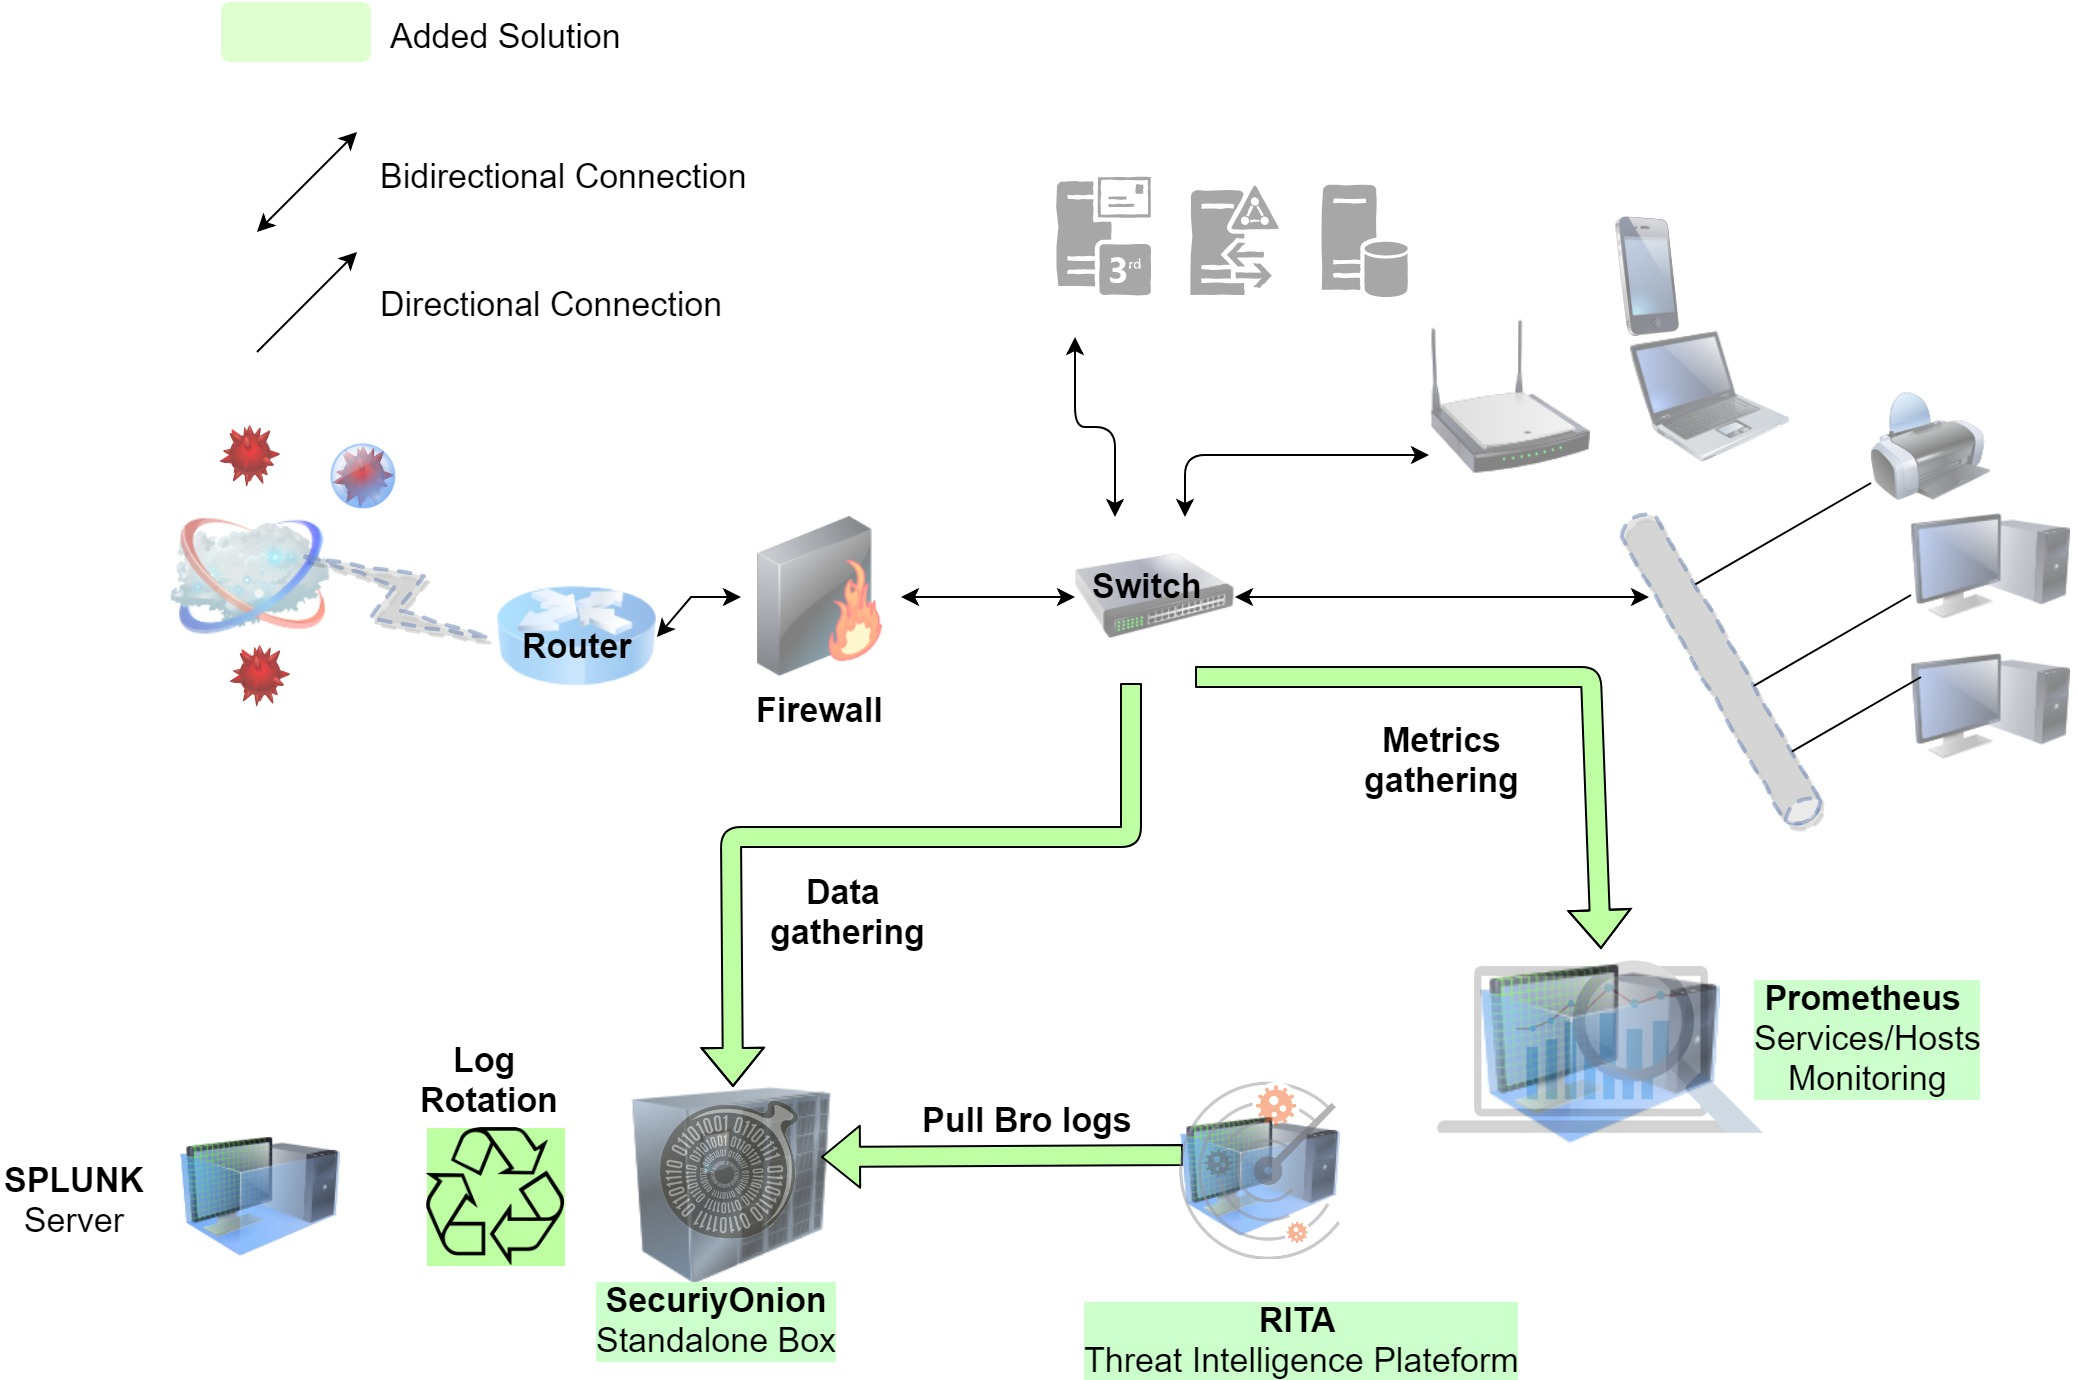
\includegraphics[width=6.3 in]{images/ATHENANewNetworkarch.jpg}
    \caption{Physical Architecture}
    \label{physic_arch}
    \end{center}
    \end{figure}~
    \item\textbf{SPLUNK Server:}
    
    SPLUNK server is already is already implemented in ATHENA, so we are going to use it in the log-rotation process(an automated process used in system administration in which dated log files are archived).
    \item \textbf{Prometheus Server:}
    
    It is a monitoring system and time series database. Placed to receive or gather metrics(internationally adopted decimal system.)
    \item \textbf{ATHENA's Endpoints:}
    
    Servers and workstations running different operating systems. Configured to send metrics to provide detailed information about system or services activity to Prometheus Server.
\end{itemize}




\section{Logical architecture}

In order to plan and understand the global design of our project, a detailed logical architecture is necessary. whose purpose is to achieve a clean separation between the components.

\subsection{SecurityOnion Box}

Figure \ref{logic_archso} illustrate SecurityOnion's main components interactions. The next paragraphs represents those components and their relations :

\begin{itemize}
    \item\textbf{Intrusion detection systems } 
    
    Network and Host IDS are placed on the bottom as they represent the first layer that is responsible for detection and alert generation based on configurable rules and scrips. Network IDS are receiving data on the network from a tool called Netsniff-ng, Host based IDS pulls processes and host activity logs from Sysmon and OSSEC agents or Syslog servers placed in Endpoint workstations or servers.
    \item\textbf{ElasticSllaearch-Logstash-Kibana }
    
    The Elastic stack is the combination of Logstash, Elasticsearch, Kibana responsible respectively of index, storage/search and visualisation of alerts and events. Curator helps Elasticsearch organise indices, Elastalert help manage alerts over the time.
    \item\textbf{Docker systems }
    
    It is a software-as-a-service tool that enables users to publish and share container-based applications through a common library. The Elastic Stack in our solution is deployed in containers and docker images.
\end{itemize} 
\begin{figure}[!htpb] 
\begin{center}
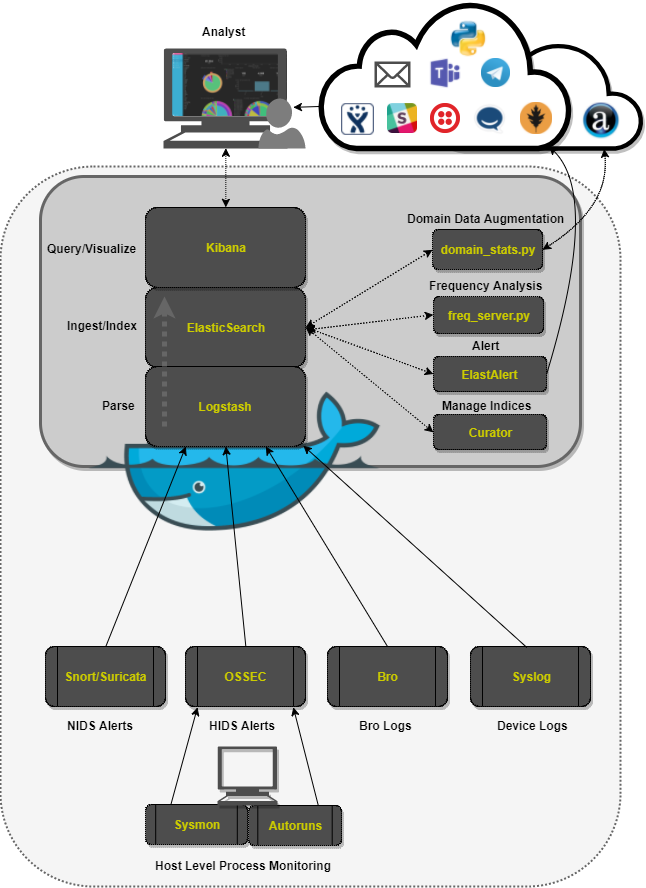
\includegraphics[width=6.3 in]{images/best_arch_so_far.png}
\caption{SecurityOnion Logical Architecture}
\label{logic_archso}
\end{center}
\end{figure}~

\newpage
\subsection{Prometheus Server}
Figure \ref{logic_archpro} illustrate metrics monitoring server's main components interactions. The next paragraphs represents those components and their relations :


\begin{figure}[!htpb] 
\begin{center}
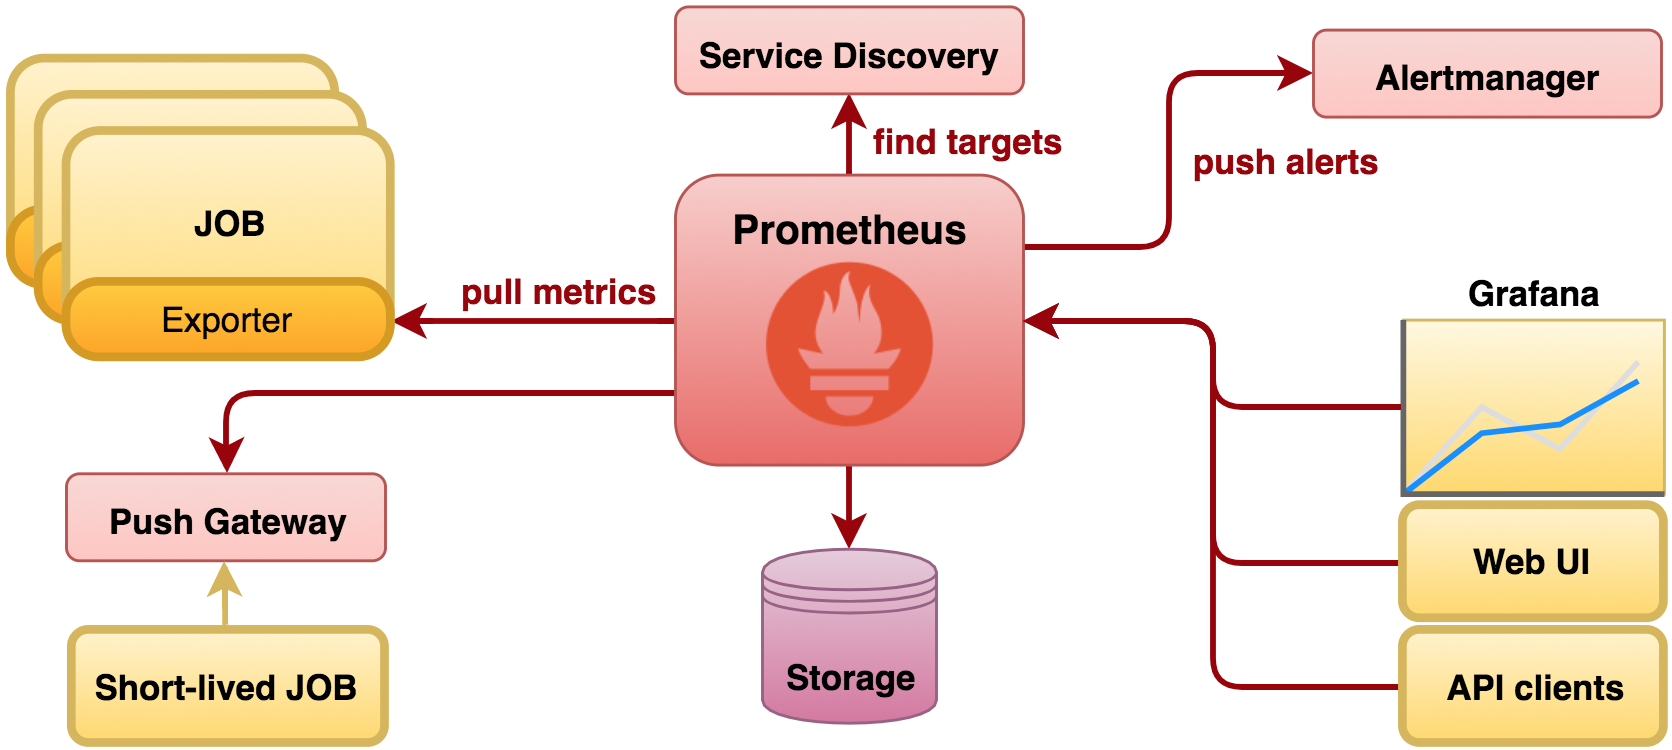
\includegraphics[width=6.0 in]{images/ATHENAprom-arch.png}
\caption{Prometheus's Logical Architecture}
\label{logic_archpro}
\end{center}
\end{figure}~

\begin{itemize}
    \item\textbf{Prometheus:}
    
    Prometheus is an open-source monitoring system with a dimensional data model, flexible query language, efficient time series database and modern alerting approach. Targets (it can be services or jobs) are registered to export metrics to Prometheus, Prometheus comes with a configurable Alertmanager responsible for user's notification in case of failures.
    \item\textbf{Grafana:}
    
    We are using Grafana as the data visualization and monitoring with support for Prometheus. Prometheus's gathered metrics are visualized in graphs and tables with Grafana.
\end{itemize}
%------------------------------------------------





\subsection *{Conclusion}
Through this chapter, we displayed the general architecture of our application. We explained subsequently the choice of our logical and physical architecture. In the next chapter, we present and expose the technologies employed during the process of creating our toolkit along with the added functionalities.




%-----------------------------------------chapter5 Achievement

\chapter {Achievement}
\renewcommand{\chaptername}{Chapter}

~~~~~This chapter discusses the implementation of the toolkit’s components.

We begin by presenting the development tools supporting the choices made then proceed to the software environment and end the chapter by displaying some interfaces of the achieved work.
\section{Developing Environment}


\subsection {Hardware Environment}
All along this project, with a reliable Internet connection, we used a computer with characteristics provided in Table \ref{computers}


\begin{table}[!htbp]

\begin{center}
\begin{tabular}{| m{5em} | m{6cm} | }
\hline
Processor & i7 2.7 GHz \\ 
\hline
Ram & 8 GB\\ 
\hline
Hard Drive & 1 TB  \\ 
\hline
Operating system & SecurityOnion 14.04 64Bits
\hline
\end{tabular}
\label{computers}
\end{center}
\caption{Characteristic of the used computer}
\end{table}


\subsection {Software Environment}
In this part, we list the different software products we used throughout the development of our application : 


%-----------------------------------------------


  
\begin{itemize}[label=\ding{112}]
  
\item\textit{Ruby Mine}

A smart editor that enables the user to produce high-quality code more efficiently, thanks to first-class support for Ruby and Rails, JavaScript and CoffeeScript, ERB and HAML, CSS and more.

Moreover, the programmer might take advantage of language specific-aware syntax \& error highlighting, code formatting, code completion, and quick documentation.
It only takes one click to switch to the declaration, super method, test, usages, implementation...
Automated yet safe refactorings are provided. They help clean the code and keep it more maintainable. Rails-aware refactorings help  performing project-wide changes: for example renaming a controller will also rename helper, views and tests. \cite{ruby}

Figure \ref{rubymine} shows an overview of RubyMine, which was the main editor we used throughout the programming phase. This software simplified the manipulation of the project's documents, syntax errors detection and server administration.
Furthermore, a few of its pre-configured features such as VCS management and included terminal were extremely proficient.

\begin{figure}[!htpb] 
\begin{center}
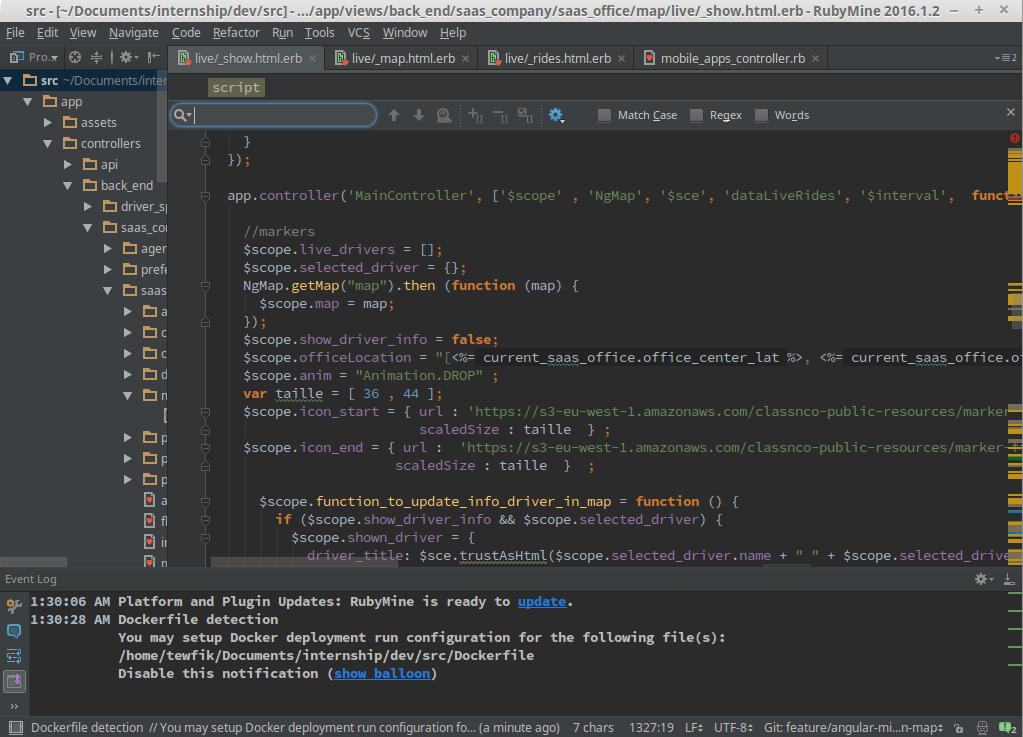
\includegraphics[width=6 in, height = 2 in]{images/rubymine.png}
\caption{RubyMine}
\label{rubymine}
\end{center}
\end{figure}



\item\textit{pgAdmin III}

pgAdmin is the most popular and feature rich Open Source administration and development platform for PostgreSQL, the most advanced Open Source database in the world. The application may be used on Linux, FreeBSD, Solaris, macOS and Windows platforms to manage PostgreSQL 9.2 and above running on any platform, as well as commercial and derived versions of PostgreSQL such as EDB Postgres Advanced Server.

pgAdmin is designed to answer the needs of all users, from writing simple SQL queries to developing complex databases. The graphical interface may be run on the desktop or on a web server and supports all common PostgreSQL features. The application includes a syntax highlighting SQL editor.

pgAdmin is developed by a community of PostgreSQL experts around the world. It is Free Software released under the PostgreSQL License. Figure \ref{pgAdmin} \cite{pgAdmin} unveils the welcome page of this software.

\begin{figure}[!htpb] 
\begin{center}
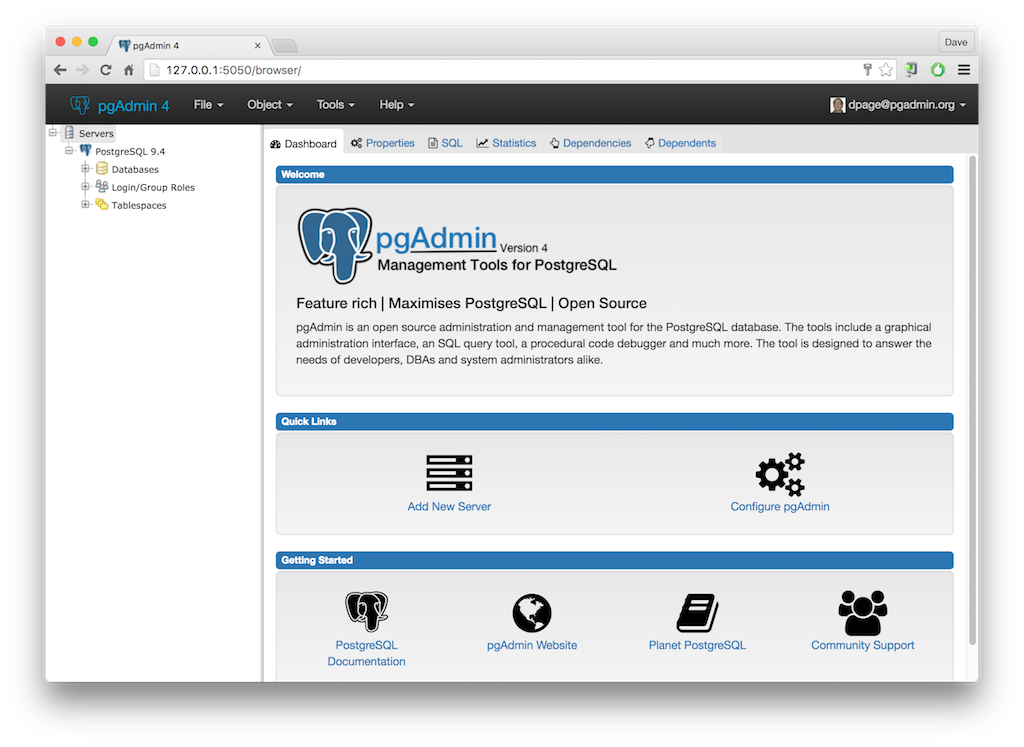
\includegraphics[width=6 in, height = 2 in]{images/pgAdmin.png}
\caption{ pgAdmin - Management Tools for PostgreSQL }
\label{pgAdmin}
\end{center}
\end{figure}

\item\textit{Draw.io}

draw.io is a free to use online diagramming application. Diagrams are then stored locally in order to edit them. We used this tool in order to draw various existing diagrams in the report. 

\item\textit{Chromium developer’s tools}

The Developer Tools, bundled and available in Chrome, grant web developers and programmers deep access into the internals of the browser and their web application.

The Developer Tools are heavily based on the WebKit Web Inspector, a part of the open source WebKit project.



Figure \ref{chrome_dev} shows an overview of the Developer Tools, points out its most popular and useful features. This tool helped us manipulating scripts, debugging as well as identifying any errors that might have occurred during the development process.

\begin{figure}[!htpb] 
\begin{center}
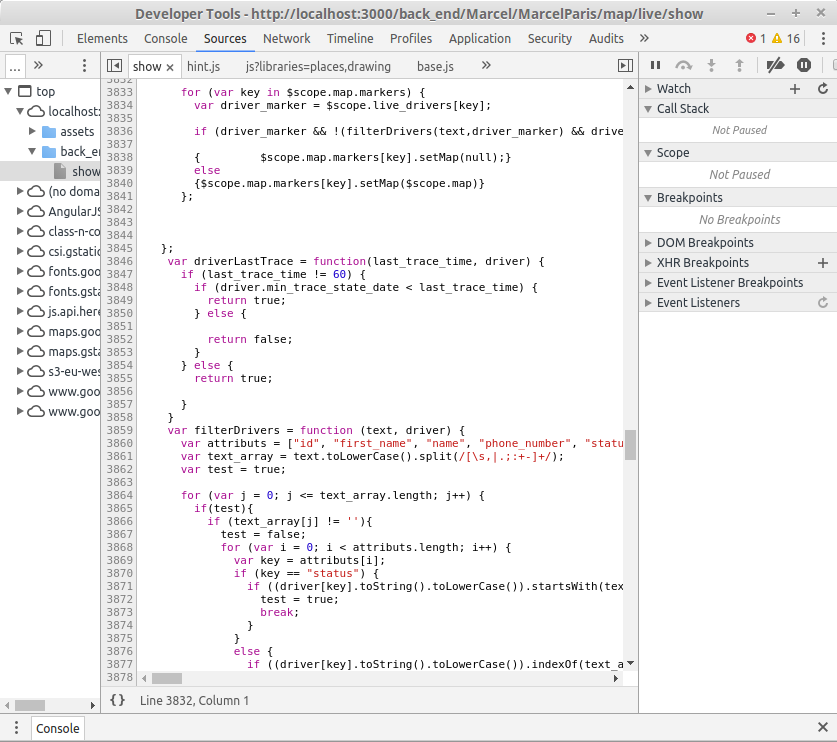
\includegraphics[width=6 in, height = 2 in]{images/chrome.png}
\caption{Chromium developer’s tools}
\label{chrome_dev}
\end{center}
\end{figure}~




%-------------------------------------
\end{itemize}



\section {Technical Choices}
In this section, we discuss the technical choices we made to achieve our application. We start
by presenting the languages used in the development of the project. Afterwards, we defend
our choice for the frameworks we used.
\subsection{Development Language}

The languages we used throughout the development phase are :
 \textbf{Shell} 

 \textbf{JavaScript } 
 
A scripting language object oriented mainly used in web browsers to add interactivity to HTML pages. In contrast to server-side languages (running on the site), JavaScript code is usually embedded directly into these pages since JS is an interpreted language meaning that scripts are executed without preliminary compilation. The standardized version of JavaScript is ECMAScript \cite{js}.

In our case, we resorted to using this programming language considering that angularJS 1.4.3 is written solely in Javascript.

\textbf{PL/pgSQL  }

PL/pgSQL (Procedural Language/PostgreSQL) is a procedural programming language supported by the PostgreSQL ORDBMS. It closely resembles Oracle's PL/SQL language.

PostgreSQL is an object-relational database management system (ORDBMS) based on POSTGRES, Version 4.2, developed at the University of California in the computer science department of Berkeley. 
In addition, PostgreSQL can be extended in several ways by the user, providing more power and flexibility.  \cite{postgres}

PostgreSQL can be used, modified and distributed by anyone for free thanks to its free licence. Regardless of these advantages, we opted for this choice since it has already been in use at the company.

\subsection{Development Framework}

The frameworks we used throughout the implementation stage are :

\begin{itemize}
\item \textbf{AngularJS } 

AngularJS is a Javascript framework. It allows the user to extend HTML vocabulary for his application. The resulting environment is extraordinarily expressive, readable and quick to develop. The main purpose of using AngularJS is promptly building responsive SPA. As a matter of fact, treating interactivity as a native component of HTML is one of the most efficient aspect of this framework.

The essential goal is building CRUD style business applications. Increasing the use of two-ways data bindings and dependency injections empowers the exploitation of angular.
Below are a few of the used modules in addition to the created ones :

\begin{itemize}[label=\ding{50}]

\item\textit{ng-map }

A module created by allenhwkim using different approach than the official module for google Maps Javascript API, since it exposes all original Google Maps V3 api to the user. It provides a simple API for diving into common map processing tasks such as setting itineraries, drawing markers, changing the type of the map, showing roads and more.. ng-map is used in the client side to ensure a fast representation process for each received ride information. Furthermore, customized markers according to the driver's type are easily incorporated into the map.


\item\textit{ui-grid }

A module created as part of AngularUI suite, the companion suite to the angularJS framework. It provides basically a data grid along with numerous features related to customizing the grid. Performing well with very large data sets as well as offering various fancy options elect it as the most suitable choice in our case. Hence, displaying wide range of ride information is handled easily by this module. Different columns adjusting options are offered as well through a user friendly and intuitive interface, while hiding the complexity of the processes.  


\item\textit{angular-animate}

Provides animation hooks for common directives such as ngRepeat, ngSwitch, and ngView, as well as custom directives via the \$animate service. These animation hooks are set in place to trigger animations during the life cycle of various directives and when triggered, will attempt to perform a CSS Transition, CSS Keyframe Animation or a JavaScript callback Animation (depending on if an animation is placed on the given directive). Animations can be placed using vanilla CSS by following the naming conventions set in place by AngularJS or with JavaScript code when it's defined as a factory \cite{ngAnimate}.

We ought to utilise ng-animate in contemplation of satisfying non functional requirements concerning the ergonomy of the application. 
Therefore, the SaaS office would enjoy a pleasant experience and dynamic interactions while manoeuvring through the application. 

\end{itemize}

\item \textbf{Twitter Bootstrap } 

Sleek, intuitive, and powerful front-end framework for faster and easier web development.

\end{itemize}


%--------------------------interfaces 
\section{Achieved Work}

In order to be successful, an application should adopt fluent and easy to follow instructions.

Especially in our case, since it consists of a SaaS product, each client insists on following his own preferences. Nevertheless, our achieved work must provide generic features that are common to all the clients. In order to ensure their satisfaction, we present in this section the different aspects of our SPA that they can easily manipulate.

\subsection{Main Page }

For starters, the SaaS office must sign in to the BackEnd workspace after inserting his credentials. Once authenticated, the main page is loaded once for all as shown in Figure \ref{int0}. He may operate on this single page application and benefit from all of its features without reloading it.

Intuitive tabs are available to ensure the ease of the use. These tabs are customizable as the user can modify their dimension, place and color as he pleases. 
The main three tabs of our component reside in 'The Map', 'The ride table' and 'The Ride Information'.

Each tab possess its own independent particularities. Yet, they are thoroughly interconnected as a constant communication between them is established.



\begin{figure}[!htbp] 
\begin{center}
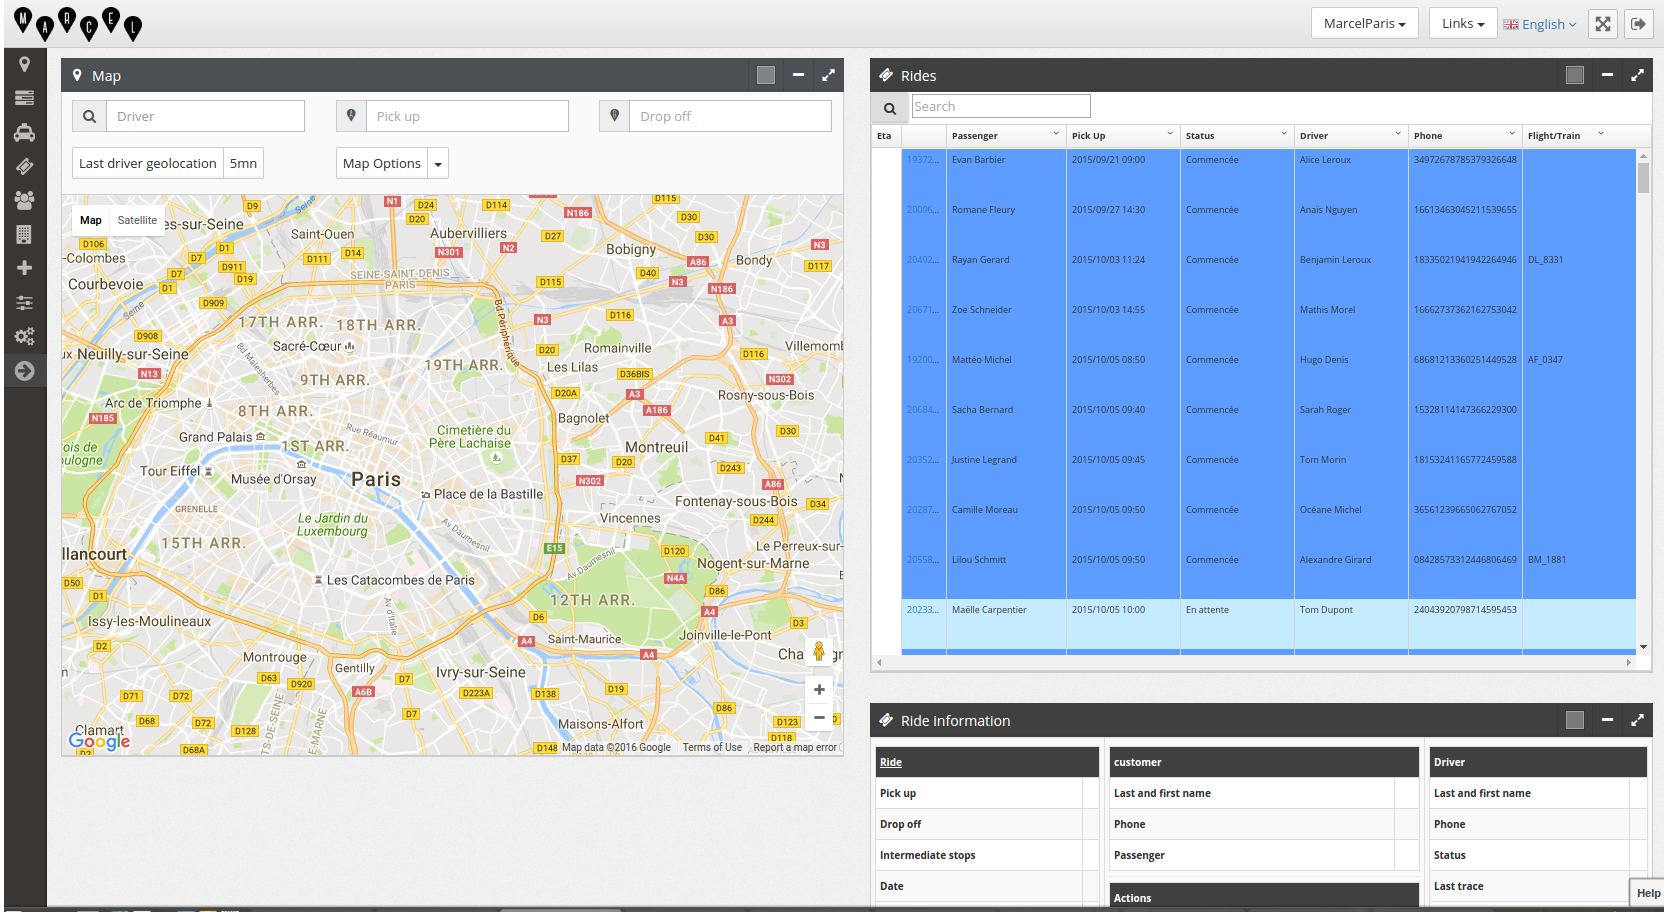
\includegraphics[width=6.6 in , height=4.5 in]{images/achievement/0.png}
\caption{Interface of the main page}
\label{int0}
\end{center}
\end{figure}~


\subsection{The Map }

The map generated by google proffers to the user all of the main aspects concerning the manipulation of the map. For instance, the user may zoom in and out and navigate through the map.
Furthermore, the user has the ability to customize the style of the map according to his preferences. The first step is to select the map styles menu that enlists the different customized styles as well as the main map modes. Figure  \ref{int2} demonstrates an example of the customized styles called 'nightvision'.

Moreover, the map's type chosen once by the user is registered in the browser session storage. So that after each reload, that saved value is assigned automatically to the map.


\begin{figure}[!htbp] 
\begin{center}
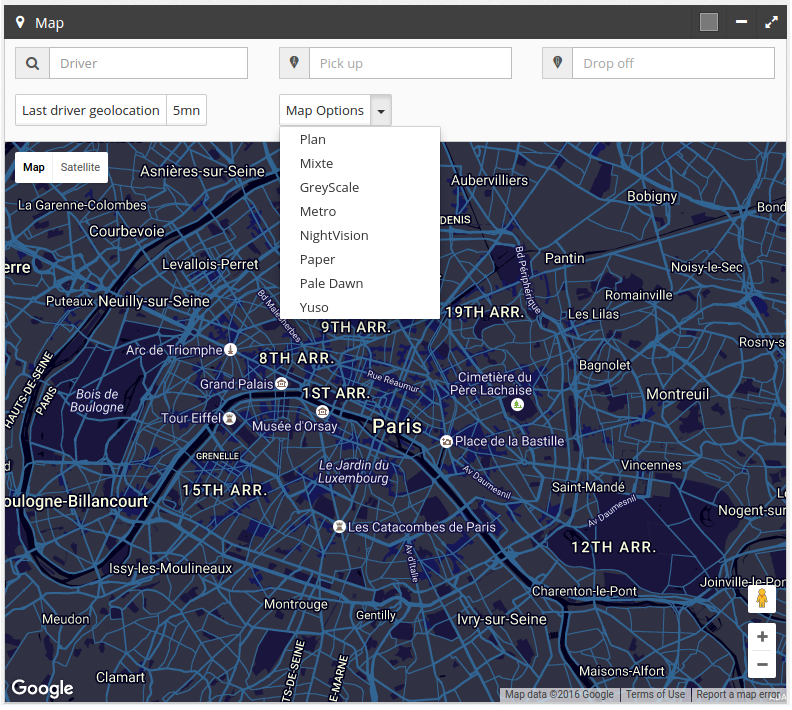
\includegraphics[width=6 in]{images/achievement/2.png}
\caption{Interface of the map tab}
\label{int2}
\end{center}
\end{figure}~

\subsection{Rides' Table }

Concerning the table of booked rides, it is filled instantly after the reload and the user may navigate through its rows.
Each row has a background color based on the status of the rides. The different colors are not specified since this was not a generic task. As a matter of fact, each client prefer different colors associated to the rides' status.

Figure \ref{int3} proves that only necessary data are displayed. These data concern the passenger's name, the pick-up time, the driver's name and phone number, the ride reference...

\begin{figure}[!htbp] 
\begin{center}
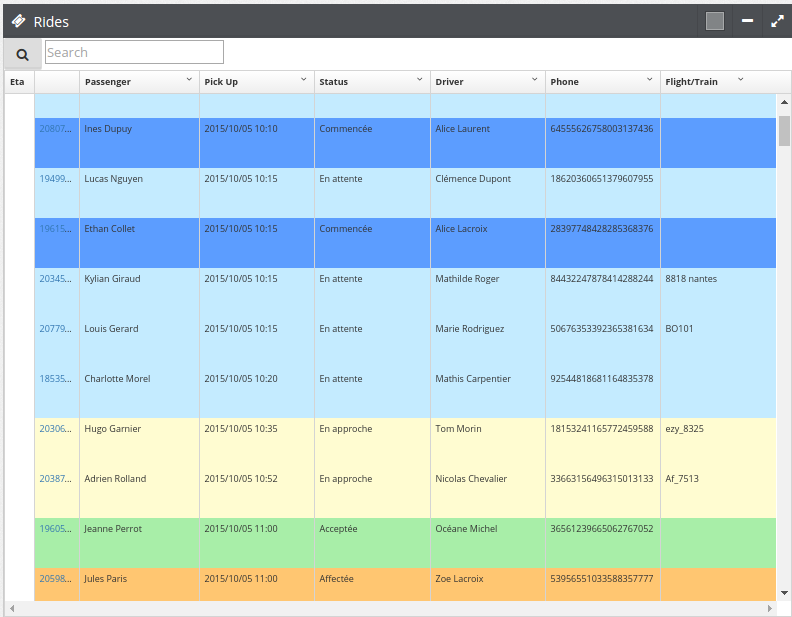
\includegraphics[width=6 in]{images/achievement/3.png}
\caption{Interface of the rides' table}
\label{int3}
\end{center}
\end{figure}~


After organizing the columns whether by descending or ascending order, the user is also able to search through the table.

Figure \ref{int4} shows that only two rows were left in the table according to the searched term. It is important to point out that the search process implies not only the passenger's name, but all of the columns. 
Hence, a view of only on-going rides is simply possible. Once the search term is to be inserted, the filter mechanism starts immediately.

\begin{figure}[!htbp] 
\begin{center}
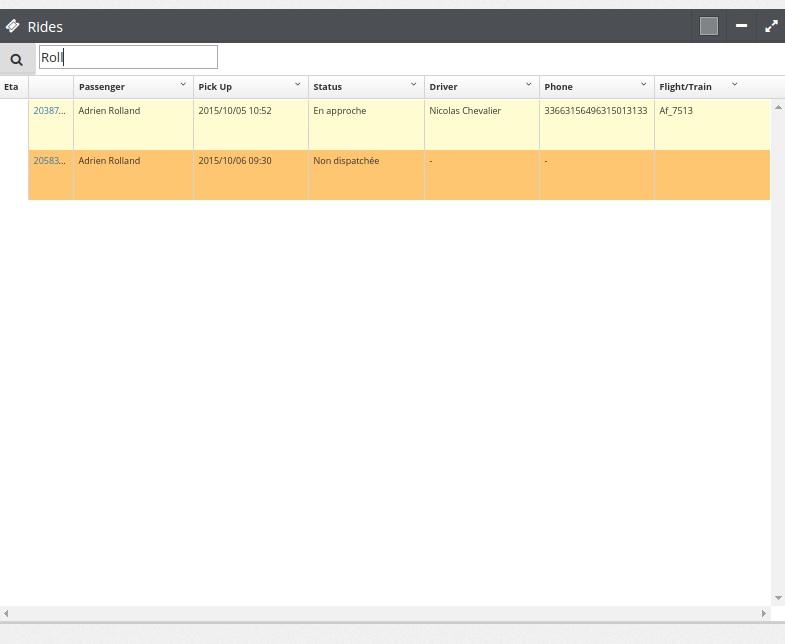
\includegraphics[width=4.5 in]{images/achievement/4.png}
\caption{Interface of the rides' table filtered }
\label{int4}
\end{center}
\end{figure}~



\subsection{Select a Ride  }

Taking a closer look at the rides' table, essential facts about the itinerary seem to be missing. Furthermore, more detailed information are being hidden in order to ensure the readability of the table.
Thus, the user is capable of reviewing the totality of information about a certain ride once he selects it. 
Simply put, the user ought to select a row in order for its background-color to change, but most importantly, further hidden data are to be shown instantly.

At this point, the user has the privilege to visualize a clear and obvious itinerary as shown in Figure \ref{int5}. In fact, the path is drawn immediately on the map with markers of the arrival and departure positions. The map is automatically zoomed into the ranged zone of the correspondent path.


\begin{figure}[!htbp] 
\begin{center}
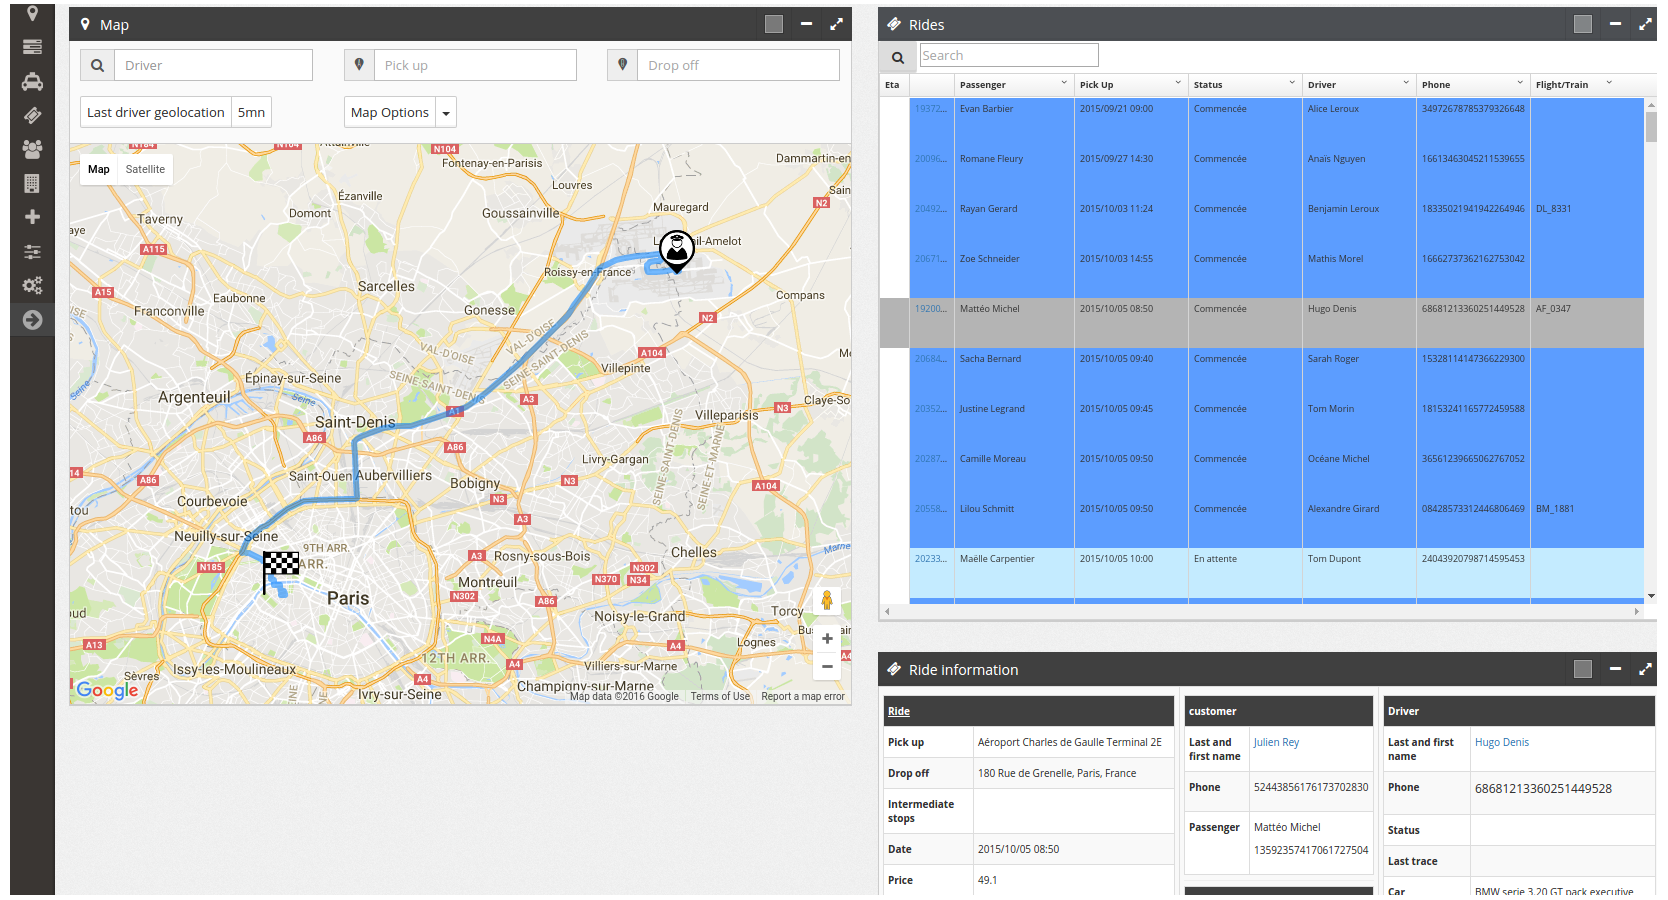
\includegraphics[width=6 in]{images/achievement/5.png}
\caption{Interface of the ride's itinerary }
\label{int5}
\end{center}
\end{figure}~


Simultaneously, the ride's information tab is instantly filled with information according the ride selected. Figure \ref{int6} shows a simple overview of the consequences of the user's click. Highlighted data such as the driver's  name and so are not just raw pieces of data. However, they constitute hyperlinks that enable the user to view their correspondent, full options, profiles. 

In addition to that, the user is only allowed to select one row at a time. Therefore, while selecting another ride, the same process is achieved again right away.



\begin{figure}[!htbp] 
\begin{center}
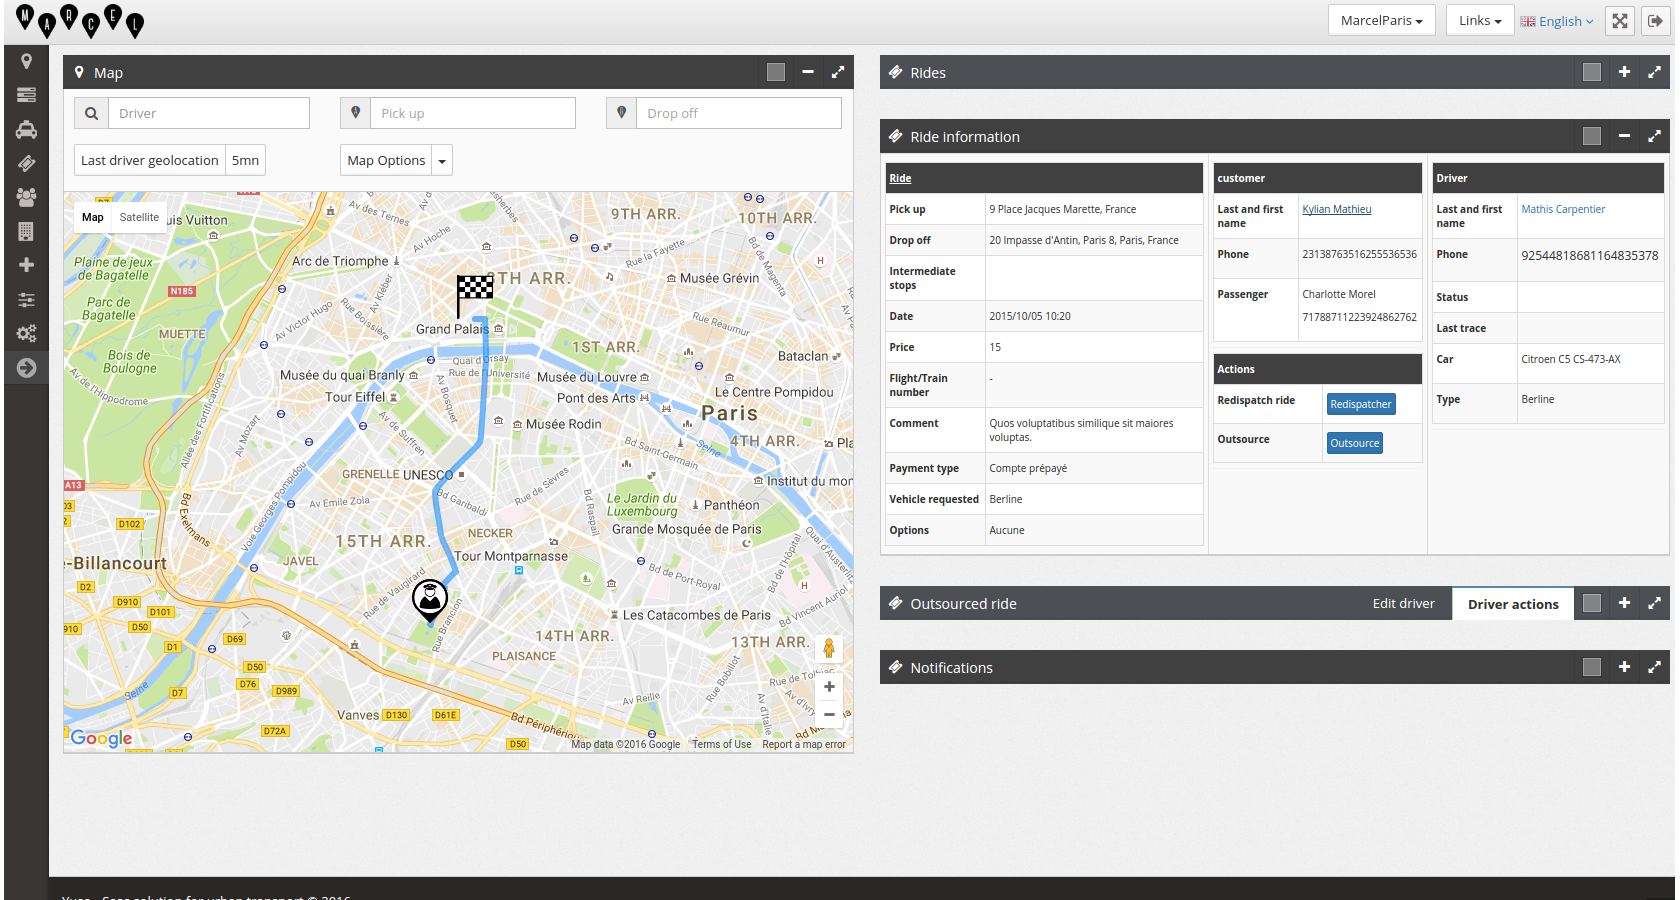
\includegraphics[width=6 in]{images/achievement/6.png}
\caption{Interface of the ride's information display }
\label{int6}
\end{center}
\end{figure}

\newpage


\subsection{Live Drivers}

The main aspect of our application is to control and view drivers in real time, hence, the user owns the entitlement of observing geolocated drivers. In fact, the drivers are being constantly geolocated through the same solution.

Meanwhile, their positions are shows as markers on the map of the all of the members of their SaaS company. Figure \ref{int1} is all about the map filled with dispersed pins. Those pins represent the drivers according to their specification.

~

\begin{figure}[!htbp] 
\begin{center}
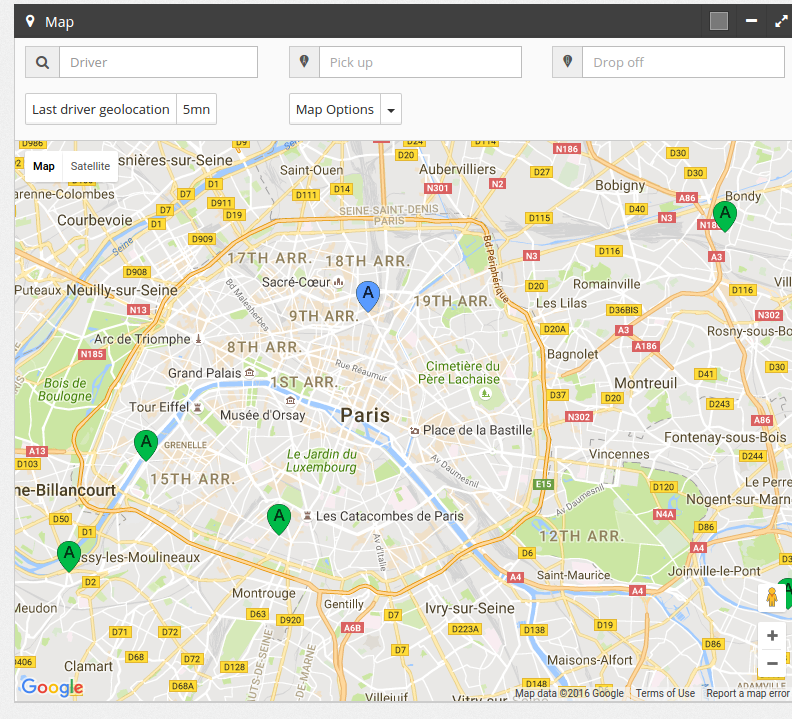
\includegraphics[width=6 in]{images/achievement/1.png}
\caption{Interface of the map with live drivers}
\label{int1}
\end{center}
\end{figure}~

The pins change their positions as the geolocalization is a continuous process. Every second the pins are alternated following the recent characteristic collected from the server. An overview of some rules are summarized in Table 5.2. The colors are standard for each client. Nevertheless, the letter written on the pin depends on the vehicle's type.



\begin{table}[!htbp]
\begin{center}
\noindent\begin{tabular}{| m{33em} | m{2cm} | }
\hline
Status & Pin \\
\hline
Started & 
\includegraphics[width=0.2 in]{images/pins/started.png} \\ 
Available & 
\includegraphics[width=0.2 in]{images/pins/dispo.png}  \\ 
Unavailable & 
\includegraphics[width=0.2 in]{images/pins/indispo.png}  \\ 
Accepted & 
\includegraphics[width=0.2 in]{images/pins/accepted.png}  \\ 
On the way & 
\includegraphics[width=0.2 in]{images/pins/way_to.png}  \\ 
On hold & 
\includegraphics[width=0.2 in]{images/pins/wait.png} \\  
Pause  & 
\includegraphics[width=0.2 in]{images/pins/pause.png}  \\ 
Soon-to-clear & 
\includegraphics[width=0.2 in]{images/pins/soon-to-clear.png}  \\  
Selected &  
\includegraphics[width=0.2 in]{images/pins/selected.png}   \\ 
Not dispatched/ Dispatched/ Dispatched Frozen/ Affected & 
\includegraphics[width=0.2in]{images/pins/not_dispatched-dispatched-dispatched_frozen-affected.png} \\ 
\hline
\end{tabular}
\end{center}
\label{pins}
\caption{Types of drivers' markers}
\end{table}




After surveying the markers, the user has also the possibility of selecting a single pin to the extend of displaying further information. As Figure \ref{int7} exhibits, a small box is displayed in the bottom of the map, listing some basic information about the driver, as well as the last geolocation time. Moreover, the color of the selected pin is changed with the preservation of the previous color. The focused pin is then highlighted and the map is zoomed around its range zone. 

Besides, the box may be hidden by a simple deselection of the chosen pin. But also, the possibility of selecting another pin while the box is active is also available. In that case, the information are changed instantly according to the new pin, and the new pin is highlighted and zoomed in like the previous one.
The old pin retrieves then its previous color either way.

\begin{figure}[!htbp] 
\begin{center}
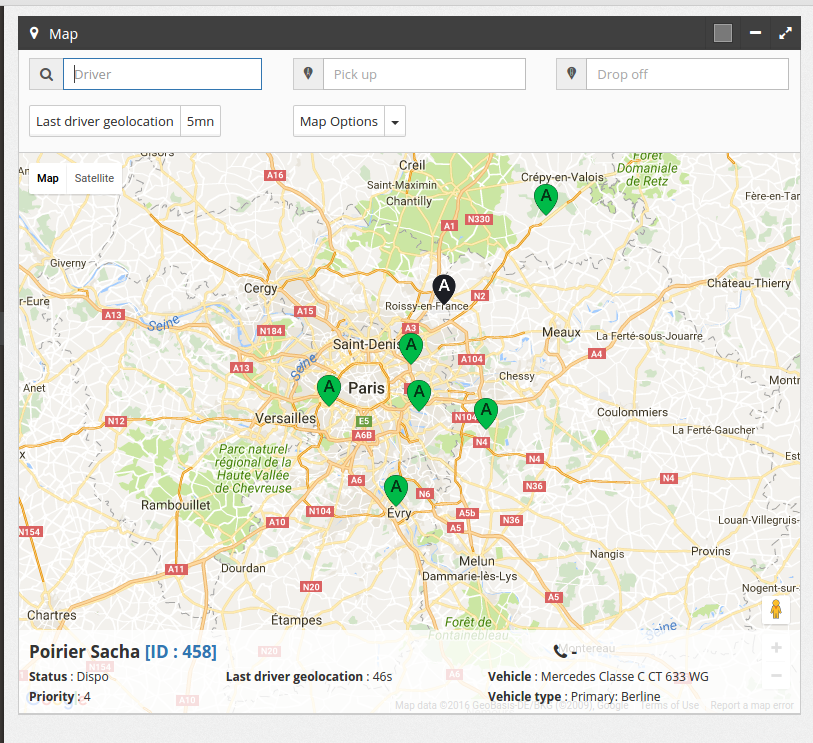
\includegraphics[width=5.8 in]{images/achievement/7.png}
\caption{Interface of the map with a selected driver}
\label{int7}
\end{center}
\end{figure}

\newpage


A few other options are mandatory in order to retrieve live driver quickly. Actually, the user may filter the driver by their last geolocation time. A menu composed of certain time intervals is available in order to hide the pins of the drivers that exceeded the time set by the user. However, pins that match the requirement are instantly shown on the map.

Furthermore, the user may search for specific set of pins by inserting various arguments. The user may input the driver's name, the pick-up and the drop-off addresses. For instance, Figure \ref{int8} demonstrates a research by the name of 'Henry'. The only marker left is by the name of Henry and has been geolocated for 37 seconds which is less than 5 minutes.

~

\begin{figure}[!htbp] 
\begin{center}
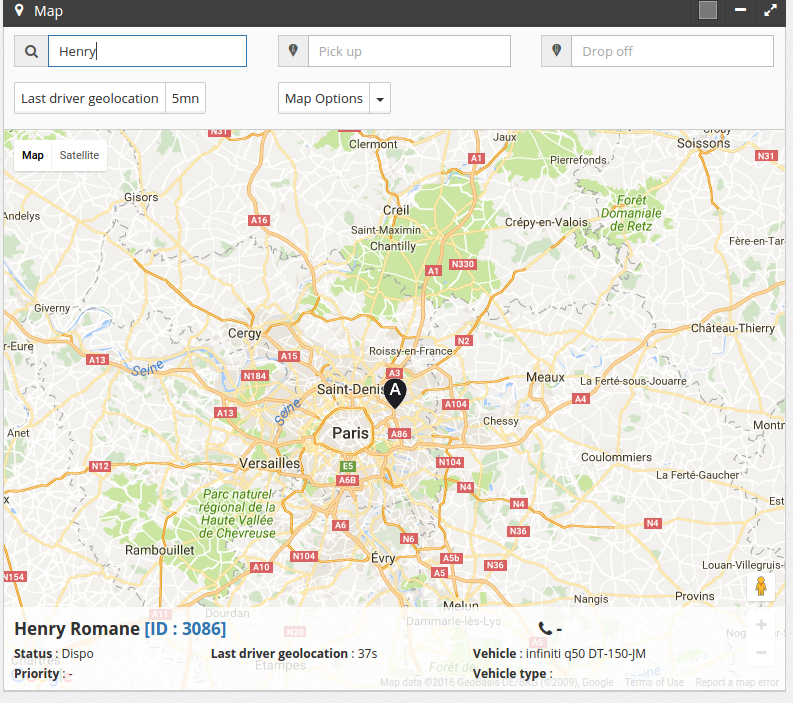
\includegraphics[width=6 in]{images/achievement/8.png}
\caption{Interface of map with filtered driver}
\label{int8}
\end{center}
\end{figure}~

~~


To wrap things up, each feature will not reduce the efficiency of an other feature, owing to the fact that, the implementation process made sure that they can work together in a harmony. Parallel procedures may occur without the need to worry about misleading results. And finally, the system has the capability to perform all of the operations simultaneously in order to provide faster and more precise information to the user.

\subsection *{Conclusion}
During this chapter, we presented the technologies that were chosen to implement our project and we argued that choice. We also presented the framework that was used and we finished by displaying the main features and interfaces of our application.








%------------------------------------------General Conclusion
\chapter*{General Conclusion}
\addcontentsline{toc}{chapter}{General Conclusion} 


\lettrine{A}s it is said, necessity is the mother of invention. In fact, men have devoted themselves through different circumstances into inventing and creating numerous types of accessories and software applications that are beneficial to their own sake. These inventions have always been in pursuance of facilitating and simplifying daily activities.

As for our case, we were interested into expediting and forwarding processes related to fleet management companies. As a matter of fact, we implemented a web component included in an automated fleet dispatching solution. This solution is being improved constantly and our component had its beneficial impact on the user's experience. 
Despite the variety of the clients' preferences, this component proffers generic features that are common to every client. Hence, they are prone to ensure better control and review of their fleet operations.


In addition to that, the new single page application is totally intuitive and easy to use, to the extend of reaching the area of interest of more clients. Being able to observe drivers on the map as well as detecting users' itineraries may turn out to be fruitful as the user is able to keep track of the company's vehicles. But most importantly, he is capable of elaborating statistics concerning the rides booked. Therefore, extensive research in order to deepen the company's knowledge about local citizens' preferences is now attainable. Afterwards, strategic plans are to be put in place straight to prioritize citizens with transportation's high-demand.


As every project can be enhanced and expanded, various perspectives are imminent for our project. We can mention the enhancement of the rides table to the extent of delivering precise required pieces of information.
Moreover, an interesting feature would be to enable the user to leave a comment in the form of a note in order to evaluate the ride, visible by other SaaS offices. 


Last but not least, we may empower our application by automatically generating statistics concerning active zones. The system would be able to recommend certain region in order to increase the number of vehicle bookings.


%----------------------------------------Bibliography & Netography
\chapter*{Bibliography}
\addcontentsline{toc}{chapter}{Bibliography} % to add it to the tables of contents



~~~~[B1]  IBM - IBM Smart Storage Cloud - United States - April 2016 - 180 P

[B2]  Alper Dincer , Balkan Uraz - Google Maps JavaScript API Cookbook - Bimingham UK - January 2013 - 316 P

[B3] Susanne Vernersson - Penetration Testing in a Web Application Environment - Sweden - October 2010 - 67 P
 
[B4] Chandermani - AngularJS by Example - United Kingdom - March 2015 - 434 P



\renewcommand\bibname{Netography}

\begin{thebibliography}{9}
\addcontentsline{toc}{chapter}{Netography} % to add it to the tables of contents



%---------------------chap0
\bibitem{linkedin}
https://www.linkedin.com/company/yusofleet (Last visit 10/10/2016 )

\bibitem{yuso}
http://www.yusofleet.com/en/ (Last visit 16/08/2016 )

\bibitem{marcel}
https://classnco-release.herokuapp.com/reservation (Last visit 10/10/2016 )

\bibitem{careme}
https://car-e-me.classnco.com/reservation (Last visit 10/10/2016 )

\bibitem{lilicab}
https://lilicab.yusofleet.com/reservation (Last visit 10/10/2016 )

\bibitem{citybird}
https://citybird.classnco.com/reservation (Last visit 10/10/2016 )

\bibitem{ocab}
https://ocab.classnco.com/reservation (Last visit 10/10/2016 )


%---------------------chap1
\bibitem{w3school}
http://www.w3schools.com/js/js\_htmldom\_methods.as (Last visit 27/07/2016 )

\bibitem{json}
https://en.wikipedia.org/wiki/JSON (Last visit 27/07/2016 )

%---------------------chap2

%---------------------chap3
%---------------------chap4

\bibitem{ruby}
https://www.jetbrains.com/ruby/ (Last visit 14/10/2016 )

\bibitem{pgAdmin}
https://www.pgadmin.org/ (Last visit 14/10/2016 )

\bibitem{js}
https://en.wikipedia.org/wiki/JavaScript (Last visit 27/07/2016 )

\bibitem{postgres}
https://www.postgresql.org/docs/7.3/static/user-preface.html (Last visit 03/08/2016 )

\bibitem{ngAnimate}
https://docs.angularjs.org/guide/animations (Last visit 18/08/2016 )

\bibitem{ansible}
https://www.ansible.com/overview/how-ansible-works (Last visit 13/25/2018)

\end{thebibliography}






\end{document}